%\documentclass{llncs}
\documentclass[runningheads,a4paper]{llncs}

\pagestyle{plain}
\usepackage{mdframed}
\usepackage{hyperref}
\usepackage{times}
\usepackage{amsmath,amssymb, latexsym}
\usepackage[latin1]{inputenc}
\usepackage{amsmath}
\usepackage{amsfonts}
\usepackage{amssymb}
\usepackage{commands}

\usepackage{enumerate}
\def\url{}
\usepackage{url}
\DeclareUrlCommand\UScore{\urlstyle{rm}}
\usepackage{xspace}
\usepackage{epsfig}
\usepackage{booktabs}
\usepackage{ifthen}
\usepackage{siunitx}
\usepackage{etoolbox}

\usepackage{fancybox}
\makeatletter
\newenvironment{CenteredBox}{% 
\begin{Sbox}}{% Save the content in a box
\end{Sbox}\centerline{\parbox{\wd\@Sbox}{\TheSbox}}}% And output it centered
\makeatother

\usepackage{pgfplots}
\usepackage{pgfkeys}
\pgfplotsset{width=0.38\linewidth,compat=1.11}
\usepgfplotslibrary{groupplots}

% magic from http://tex.stackexchange.com/questions/117759/create-x-and-y-label-which-overlaps-for-multiple-plots
\makeatletter
\pgfplotsset{
    groupplot xlabel/.initial={},
    every groupplot x label/.style={
        at={($({group c1r\pgfplots@group@rows.west}|-{group c1r\pgfplots@group@rows.outer south})!0.5!({group c\pgfplots@group@columns r\pgfplots@group@rows.east}|-{group c\pgfplots@group@columns r\pgfplots@group@rows.outer south})$)},
        anchor=north,
    },
    groupplot ylabel/.initial={},
    every groupplot y label/.style={
            rotate=90,
        at={($({group c1r1.north}-|{group c1r1.outer
west})!0.5!({group c1r\pgfplots@group@rows.south}-|{group c1r\pgfplots@group@rows.outer west})$)},
        anchor=south
    },
    execute at end groupplot/.code={%
      \node [/pgfplots/every groupplot x label]
{\pgfkeysvalueof{/pgfplots/groupplot xlabel}};  
      \node [/pgfplots/every groupplot y label] 
{\pgfkeysvalueof{/pgfplots/groupplot ylabel}};  
    },
    group/only outer labels/.style =
{
group/every plot/.code = {%
    \ifnum\pgfplots@group@current@row=\pgfplots@group@rows\else%
        \pgfkeys{xticklabels = {}, xlabel = {}}\fi%
    \ifnum\pgfplots@group@current@column=1\else%
        \pgfkeys{yticklabels = {}, ylabel = {}}\fi%
}
}
}

\def\endpgfplots@environment@groupplot{%
    \endpgfplots@environment@opt%
    \pgfkeys{/pgfplots/execute at end groupplot}%
    \endgroup%
}
\makeatother


%% \newcommand{\isTechReport}{false} % true or false
\newcommand{\includeProof}[1]{
  \ifthenelse{\equal{\isTechReport}{true}}{
    #1
  }{
  }
}

% command to end a proof or definition:
%\def\qed{\rule{0.4em}{1.4ex}}
\def\qed{\hfill$\Box$}

% space at the beginning of an environment:
\def\@envspa{\hspace{0.3em}}
\def\@sa{\hspace{-0.2em}}
\def\@sb{\hspace{0.5em}}
\def\@sc{\hspace{-0.1em}}

\def\sk{\smallskip}		% space before and after theorems

\newtheorem{notation}{Notation}{\itshape}{}
\newtheorem{invariant}{Invariant}

\newcommand{\isTechReport}{false} % true or false
\newcommand\includeTechRep[1]{%
  \ifthenelse{\equal{\isTechReport}{true}}
    {{#1}}
    {\ignorespaces}
\xspace}

%\usepackage{listings}
%
%\usepackage{color}
% uncomment next line to restore colors
% \def\withcolor{}

\ifdefined\withcolor
	\definecolor{haskellblue}{rgb}{0.0, 0.0, 1.0}
	\definecolor{haskellstr}{rgb}{0.2, 0.2, 0.6}
	\definecolor{haskellred}{rgb}{1.0, 0.0, 0.0}
	\definecolor{gray_ulisses}{gray}{0.55}
	\definecolor{castanho_ulisses}{rgb}{0.71,0.33,0.14}
	\definecolor{preto_ulisses}{rgb}{0.41,0.20,0.04}
	\definecolor{green_ulisses}{rgb}{0.0,0.4,0.0}
\else
	\definecolor{haskellblue}{gray}{0.1}
	\definecolor{haskellstr}{gray}{0.1}
	\definecolor{haskellred}{gray}{0.1}
	\definecolor{gray_ulisses}{gray}{0.1}
	\definecolor{castanho_ulisses}{gray}{0.1}
	\definecolor{preto_ulisses}{gray}{0.1}
	\definecolor{green_ulisses}{gray}{0.1}
\fi


\def\codesize{\normalsize}

\lstdefinelanguage{HaskellUlisses}{
	basicstyle=\ttfamily,
	sensitive=true,
	morecomment=[l][\color{gray_ulisses}\ttfamily]{--},
	morecomment=[s][\color{gray_ulisses}\ttfamily]{\{-}{-\}},
	morestring=[b]",
	stringstyle=\color{haskellstr},
	showstringspaces=false,
	numberstyle=\codesize,
	numberblanklines=true,
	showspaces=false,
	breaklines=true,
	showtabs=false,
        escapeinside={(*}{*)},%
        % mathescape=true,
	emph=
	{[1]
		FilePath,IOError,abs,acos,acosh,and,any,appendFile,approxRational,asTypeOf,asin,
		asinh,atan,atan2,atanh,basicIORun,break,catch,ceiling,chr,compare,concat,concatMap,
		const,cos,cosh,curry,cycle,decodeFloat,denominator,digitToInt,div,divMod,drop,
		dropWhile,either,elem,encodeFloat,enumFrom,enumFromThen,enumFromThenTo,enumFromTo,
		error,even,exp,exponent,fail,filter,flip,floatDigits,floatRadix,floatRange,floor,
		fmap,foldl,foldl1,foldr,foldr1,fromDouble,fromEnum,fromInt,fromInteger,
		fromRational,fst,gcd,getChar,getContents,getLine,head,id,inRange,index,init,intToDigit,
		interact,ioError,isAlpha,isAlphaNum,isAscii,isControl,isDenormalized,isDigit,isHexDigit,
		isIEEE,isInfinite,isLower,isNaN,isNegativeZero,isOctDigit,isPrint,isSpace,isUpper,iterate,
		last,lcm,length,lex,lexDigits,lexLitChar,lines,log,logBase,lookup,mapM,mapM_,max,
		maxBound,maximum,maybe,min,minBound,minimum,mod,negate,not,notElem,numerator,odd,
		or,pi,primExitWith,print,product,properFraction,putChar,putStr,putStrLn,quot,
		quotRem,range,rangeSize,read,readDec,readFile,readFloat,readHex,readIO,readInt,readList,readLitChar,
		readLn,readOct,readParen,readSigned,reads,readsPrec,realToFrac,recip,rem,repeat,
		reverse,round,scaleFloat,scanl,scanl1,scanr,scanr1,seq,sequence,sequence_,show,showChar,showInt,
		showList,showLitChar,showParen,showSigned,showString,shows,showsPrec,significand,signum,sin,
		sinh,snd,span,splitAt,sqrt,subtract,succ,sum,tail,take,takeWhile,tan,tanh,threadToIOResult,toEnum,
		toInt,toInteger,toLower,toRational,toUpper,truncate,uncurry,undefined,unlines,until,unwords,unzip,
		unzip3,userError,words,writeFile,zip,zip3,zipWith,zipWith3,listArray,doParse,for,initTo,
                create,get,set,div,rescale,add,delete,insert,prop_focus_left_master,average,best,insert,union,split,size,fromList,copy,group,good,bad,foo,explode,singleton,difference,fromJust,sort,unfold,
                subst,unapply,apply,proxy,refinement,fresh,guard,constrain,oneOf,
                queryList,queryCtor,queryField,ctors,decodeCtor,whichOf,ctorArity,eval,
                mkCtor,gCtors,gEncode,gEncodeFields,gDecode,gDecodeFields,reproxyRep,empty,splitCtor,checkField,scanM,
                padAverage,focusUp,execute,checkSMT,inputTypes,outputType,toReft,app,
                genArgs,genWitness,close,witness,mkApps,mkLets,isStuck,findExpr,updState,putBefore,putAfter,
                putRoot,getNext,getPrev,getSubterms,applyCtx,findApp,findVal,replicate,loop,fac,incAllByOne,map
                %, inTypes, inputTypes, outputType, execute, smtFindModel, smtRefuteModel
	},
	emphstyle={[1]\color{haskellblue}},
	emph=
	{[2]
		OkMap,OkRBT,OkStackSet,TTrue,Map,Bool,Char,Double,Either,Float,IO,Integer,Int,Maybe,Ordering,Rational,Ratio,ReadS,ShowS,String,Word8,Nat,Pos,Rng,Score,
                Ptr,ForeignPtr,CSize,InPacket,Tree,Prop,TreeEq,TreeLt,Vec,
                NullTerm,IncrList,DecrList,UniqList,BST,MinHeap,MaxHeap,
                PtrN,ByteStringN,ByteStringEq,VO,ByteStringsEq,ByteStringNE,OrdList,Var,RType,Constrain,Gen,Var,Proxy,SMT,Targetable,RefType,Refinement,Ctor,C1,Rep,Rec0,U1,
                GCtors,GDecode,GDecodeFields,GEncode,GEncodeFields,OrdMap,MinusKey,
                len,isBH,isBal,bh,isRB,keys,Sorted,RBT,Col,isBlack,OrdRBT,Set,sz,
                StackSet,NoDuplicates,Data,RBTree,XMonad,Generic,
                VState,Expr,Ctx,Cmd,int,list,string,bool
	},
	emphstyle={[2]\color{castanho_ulisses}},
	emph=
	{[3]
		case,class,data,deriving,do,else,if,return,def,import,in,infixl,infixr,instance,let,tmapM,for2M,forM,zipWithM,otherwise,
		module,measure,pred,predicate,of,primitive,then,type,where,lazy,throw,when,
                rec,function,fun,match,with
	},
	emphstyle={[3]\color{preto_ulisses}\textbf},
	emph=
	{[4]
		quot,rem,div,mod,elem,notElem,seq
	},
	emphstyle={[4]\color{castanho_ulisses}\textbf},
	emph=
	{[5]
		PS,Tip,Node,Black,Red,EQ,False,GT,Just,LT,Left,Nothing,Right,True,Show,Eq,Ord,Num,C,N,Leaf,Bin,CounterExample,
                StepForward,StepBack,JumpForward,JumpBack,StepOver,StepInto,true
	},
	emphstyle={[5]\color{green_ulisses}},
	emph=
	{[6]
		patError, irrefutPatError, nonExhaustiveGuardsError, recSelError, errorOut,
		noMethodBinding
	},
	emphstyle={[6]\color{haskellred}}
}

%%%ORIG
%%%\lstnewenvironment{code}
%%%{\textbf{Haskell Code} \hspace{1cm} \hrulefill \lstset{language=HaskellUlisses}}
%%%{\hrule\smallskip}

%V1
%\lstnewenvironment{code}
%{\smallskip \lstset{language=HaskellUlisses}}
%{\smallskip}

\lstdefinelanguage{HaskellUlissesMath}[]{HaskellUlisses}{mathescape=true}

\lstnewenvironment{code}
{\lstset{language=HaskellUlisses}}
{}

\lstnewenvironment{ecode}
{\lstset{language=HaskellUlisses
				,numbers=left
                                ,frame=leftline
                                ,xleftmargin=7.5mm
				,moredelim=[is][\textbf]{==}{==}
				,moredelim=[is][\underbar]{__}{__}
				}}
{}

\lstnewenvironment{mcode}
{\lstset{language=HaskellUlissesMath}}
{}

\lstnewenvironment{fcode}
{\lstset{language=HaskellUlisses, frame=L}}
{}

\lstMakeShortInline[language=HaskellUlisses]@
\lstMakeShortInline[language=HaskellUlissesMath]|


\sloppy

\title{Type Targeted Testing}
\author{Eric L. Seidel \and Niki Vazou \and Ranjit Jhala}
\institute{UC San Diego}

%% Gradual Verification via Type Targeted Testing
%% Testing with Types
%% Executing Code with Types
%% Type Symbolic System Exec
%% Type-directed Exhaustive Symbolic Testing.
%% Directed Automatic Randomized Testing
%% Type Automatic Test Generation
 

%% TARGET: Type And Refinement Guided Exhaustive Testing
%% TARGET: Type And Refinement Guided Testing
%% TARGET: Type Guided Testing
%% Testing With Types
%% Testing While Typing
%% Tests From Types
%% Turning Types Into Tests
%% Types as Tests
%% Generating Tests from Types
%% Synthesizing Tests from Types
%% Type Based Test Synthesis
%% Type Based Test Generation 
%% Type Guided Test Generation
%% Type Driven Test Generation

\begin{document}
\maketitle


\begin{abstract}
Localizing type errors is challenging in
languages with global type inference, as
the type checker must make assumptions
about what the programmer intended to do.
%
We introduce \toolname, a \emph{data-driven}
approach to error localization based on
supervised learning.
%
\toolname analyzes a large corpus
of training data --- pairs of ill-typed
programs and their ``fixed'' versions ---
to automatically \emph{learn a model}
of where the error is most likely
to be found.
%
Given a new ill-typed program,
\toolname executes the model to
generate a list of potential blame
assignments ranked by likelihood.
%
We evaluate \toolname by comparing its
precision to the state of the art
on a set of over 5,000 ill-typed \ocaml
programs drawn from two instances of an
introductory programming course.
%
We show that when the top-ranked blame assignment
is considered, \toolname's data-driven
model is able to correctly predict
the exact sub-expression that should
be changed \HiddenFhTopOne\% of the time, %which is
\ToolnameWinOcaml points higher than \ocaml and
\ToolnameWinSherrloc points higher than the state-of-the-art
\sherrloc tool.
%
Furthermore, \toolname's accuracy surpasses
\HiddenFhTopTwo\% when we consider the top \emph{two}
locations and reaches \HiddenFhTopThree\% if we consider
the top \emph{three}.
\end{abstract}

%\section{Introduction}
\label{sec:nanomaly:introduction}

% Type errors are a common stumbling block for students
% trying to learn typed functional languages like \ocaml\
% and \haskell.
% %
% Consider the ill-typed @fac@ function on the left in
% Figure~\ref{fig:factorial}.
% %
% The function returns @true@ in the base case (instead of @1@),
% and so \ocaml responds with the error message:
% %
% \begin{verbatim}
%   This expression has type
%     bool
%   but an expression was expected of type
%     int.
% \end{verbatim}
% %
% This message makes perfect sense to an expert who is familiar
% with the language and has a good mental model of how the type
% system works.
% %
% However, it may perplex a novice who has yet to develop such a
% mental model.
% %
% To make matters worse, unification-based type inference algorithms
% often report errors far removed from their source.
% %
% This further increases the novice's confusion and can actively mislead
% them to focus their investigation on an irrelevant piece of code.
% %
% Much recent work has focused on analyzing unification constraints
% to properly \emph{localize} a type error~\cite{Lerner2007-dt,Chen2014-gd,Zhang2014-lv,Pavlinovic2014-mr},
% but an accurate source location does not explain \emph{why} the
% program is wrong.


\begin{figure}[t]
\centering
\begin{minipage}{.49\linewidth}
\centering
\begin{ecode}
let rec sumList xs =
  match xs with
  | []   -> []
  | h::t -> h + (*@\hlRed{sumList t}@*)
\end{ecode}
\vspace{2em}
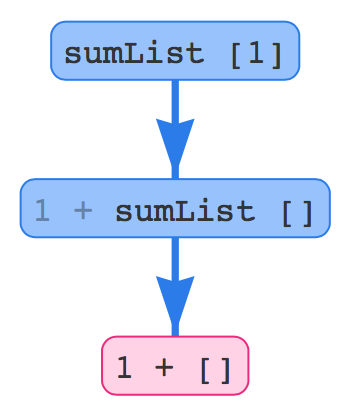
\includegraphics[height=1.5in]{nanomaly/sumList-overview.png}
\end{minipage}
\begin{minipage}{.49\linewidth}
\centering
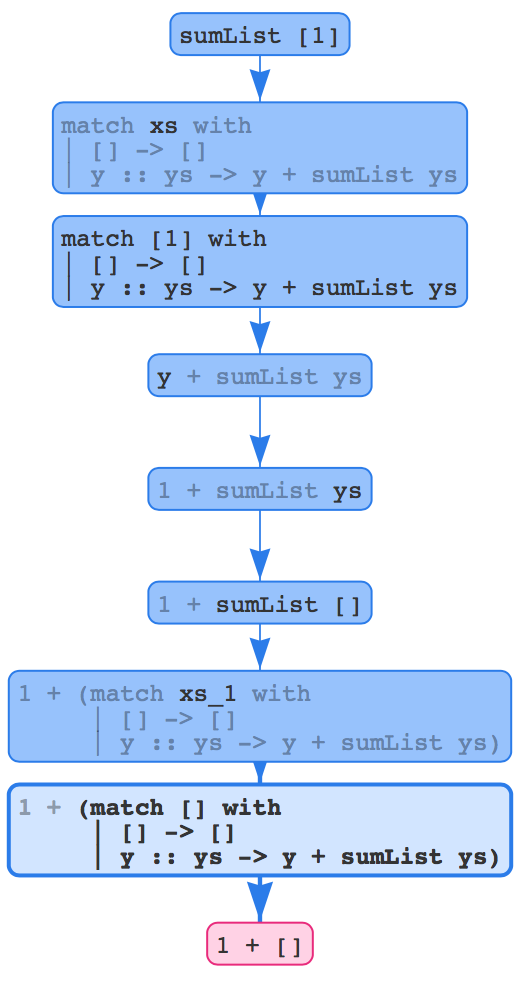
\includegraphics[height=3in]{nanomaly/sumList-long.png}
\end{minipage}
\vspace{1em}
\caption[(top-left) The ill-typed \texttt{sumList} function
  highlighting the error location reported by
  \ocaml. (bottom-left) Dynamically witnessing the type error in
  \texttt{sumList}, showing only function call-return pairs. (right) The
  same trace, fully expanded to show each small-step reduction in the
  computation.]{(top-left) The ill-typed \texttt{sumList} function
  \hlRed{highlighting} the error location reported by
  \ocaml. (bottom-left) Dynamically witnessing the type error in
  \texttt{sumList}, showing only function call-return pairs. (right) The
  same trace, fully expanded to show each small-step reduction in the
  computation.}
\label{fig:factorial}
\end{figure}

We have noticed a common theme in the existing literature on type error
diagnosis: errors are always presented in terms of the static type
system, and yet (static) type systems are meant to rule out certain
types of \emph{dynamic} errors.
%
We believe this may be particularly confusing for novice users, who must
simultaneously develop a mental model of the dynamic (evaluation)
semantics and the static (typing) semantics of the language they are
learning.
%
Furthermore, given the rise of dynamic languages like \textsc{Python}
and \textsc{Javascript} as teaching languages, novices may be more
familiar with reasoning about the dynamic semantics of a program than
the static semantics.
%
Thus, by connecting the static type error to the dynamic error it
would prevent, we might help novices understand the type system better.

In this chapter we propose a new approach that explains static type
errors by \emph{dynamically} witnessing how an ill-typed program goes
wrong.
%
We have developed \toolname, an interactive tool that uses
the source of the ill-typed function to automatically synthesize
the result on the bottom-left in Figure~\ref{fig:factorial}, which
shows how the recursive calls reduce to a configuration where
the program ``goes wrong'' --- \ie\ the @int@ value @0@ is to be
added to the @list@ value @[]@.
We achieve this via three concrete contributions.

\paragraph{1. Finding Witnesses}
Our first contribution is an algorithm for searching for
\emph{witnesses} to type errors, \ie\ inputs that cause a
program to go wrong~(\S~\ref{sec:nanomaly:searching-witness}).
%
This problem is tricky when we cannot rely on
static type information, as we must avoid the
trap of \emph{spurious} inputs that cause
irrelevant problems that would be avoided
by picking values of a different, relevant type.
%
We solve this problem by developing a novel
operational semantics that combines evaluation
and type inference.
%
We execute the program with \emph{holes} --- values whose type is
unknown --- as the inputs.
%
A hole remains abstract until the evaluation
context tells us what type it must have, for
example the parameters to an addition operation
must both be integers.
%
Our semantics conservatively instantiates holes
with concrete values, dynamically inferring the
type of the input until the program goes wrong.
%
We prove that our procedure synthesizes \emph{general}
witnesses, which means, intuitively, that if a witness
is found for a given ill-typed function, then, \emph{for all}
(inhabited) input types, there exist values that can make
the function go wrong.

Given a witness to a type error, the novice may still be at a loss.
%
The standard \ocaml\ interpreter and debugging infrastructure expect
well-typed programs, so they cannot be used to investigate \emph{how}
the witness causes the program to crash.
%
More importantly, the execution itself may be quite long and may contain
details not relevant to the actual error.

\paragraph{2. Visualizing Witnesses}
Our second contribution is an interactive visualization of the
execution of purely functional \ocaml\ programs, well-typed or not~(\S~\ref{sec:nanomaly:interactive}).
%
We extend the semantics to also build a \emph{reduction graph}
which records all of the small-step reductions and the context
in which they occur.
%
The graph lets us visualize the sequence of
steps from the source witness to the stuck term. The user can
interactively expand the computation to expose intermediate steps
by selecting an expression and choosing a traversal strategy.
%
The strategies include many of the standard debugging moves, \eg\
stepping \emph{forward} or \emph{into} or \emph{over} calls, as well
stepping or jumping \emph{backward} to understand how a particular
value was created, while preserving a context of the intermediate
steps that allow the user to keep track of a term's provenance.

We introduce a notion of \emph{jump-compressed} traces to abstract away
the irrelevant details of a computation.
%
A jump-compressed trace includes only function
calls and returns. For example, the trace in the bottom-left of
Figure~\ref{fig:factorial} is jump-compressed.
%
Jump-compressed traces are similar to stack traces in that both show a
sequence of function calls that lead to a crash. However, jump-compressed
traces also show the return values of successful calls, which can be
useful in understanding why a particular path was taken.

\paragraph{3. Evaluating Witnesses}
%
Of course, the problem of finding witnesses is
undecidable in general. In fact, due to the necessarily
conservative nature of static typing, there
may not even exist any witnesses for a given
ill-typed program.
%
Thus, our approach is a heuristic that is only useful
if it can find \emph{compact} witnesses for
\emph{real-world} programs.
%
Our third contribution is an extensive evaluation of our approach
on two different sets of ill-typed programs obtained by instrumenting
compilers used in beginner's classes~(\S~\ref{sec:nanomaly:evaluation}).
%
The first is the \uwbench\ dataset~\cite{Lerner2007-dt}, standard in the
literature, comprising \uwsize\ ill-typed programs.
%
The second comes from the new dataset described in \autoref{chp:data-collection}, comprising \ucsdsize\
ill-typed programs.
%
We show that for both datasets, our technique is able to generate
witnesses for around 85\% of the programs, in under a second in the
vast majority of cases.
%
Furthermore, we show that a simple interactive strategy yields
compact counterexample traces with at most 5 steps for 60\%
of the programs, and at most 10 steps for over 80\% of the programs.
%
We can even use witnesses to \emph{localize} type errors with a simple
heuristic that treats the values in a ``stuck'' term as \emph{sources}
of typing constraints and the term itself as a \emph{sink},
achieving around 70\% accuracy in locating the source of the error.

The ultimate purpose of an error report is to help the programmer
\emph{comprehend} and \emph{fix} problematic code.
%
Thus, our final contribution is a user study that compares \toolname's
dynamic witnesses against \ocaml's type errors along the dimension of
comprehensibility~(\S~\ref{sec:nanomaly:user-study}).
%
Our study finds that students given one of our witnesses are
consistently more likely to correctly explain and fix a type
error than those given the standard error message produced by
the \ocaml compiler.


%
% \subparagraph{Witness Utility}
%
% Even if we can find small witnesses for the majority of type errors, it
% may be that the witnesses do not actually help developers
% \emph{understand} the errors.
%
% In other words, perhaps the static error message is sufficient to
% diagnose and fix the error, or perhaps the witness simply does not add
% enough information to make a difference.
%
%
% Thus, our final contribution is a user study that compares the utility
% of our witnesses with that of the error messages provided by the \ocaml
% compiler~(\S~\ref{sec:nanomaly:user-study}).
%

\smallskip
All together, our results show that in the vast majority of cases, (novices') ill-typed
programs \emph{do} go wrong, and that the witnesses to these errors can be
helpful in understanding the source of the error. This, in turn, opens the
door to a novel dynamic way to explain, understand, and appreciate the
benefits of static typing.


%%% Local Variables:
%%% mode: latex
%%% TeX-master: "main"
%%% End:

\section{Overview}
\label{sec:overview}

We start with an overview of our approach to
explaining (static) type errors using \emph{witnesses}
that (dynamically) show how the program goes wrong.
%
We illustrate why generating suitable inputs
to functions is tricky in the absence of type
information.
%
Then we describe our solution to the problem
and highlight the similarity to static type
inference,
%
Finally, we demonstrate our visualization of
the synthesized witnesses.

\subsection{Generating Witnesses}
\label{sec:generating-witnesses}
Our goal is to find concrete values
that demonstrate how a program ``goes wrong''.

\paragraph{Problem: Which inputs are bad?}
%
One approach is to randomly generate input values and
use them to execute the program until we find one that
causes the program to go wrong.
%
Unfortunately, this approach quickly runs aground.
Recall the erroneous @fac@ function from Figure~\ref{fig:factorial}.
%~\S~\ref{sec:introduction}:
%
% \begin{code}
  % let rec fac n =
    % if n <= 0 then
      % true
    % else
      % n * fac (n-1)
% \end{code}
% \ES{having two copies of \texttt{fac} seems silly, but the back-reference across a page boundary is no good either...}
%
What \emph{types} of inputs should we test @fac@ with?
%
Values of type @int@ are fair game, but values of type, say,
@string@ or @int list@ will cause the program to go wrong
in an \emph{irrelevant} manner.
%
Concretely, we want to avoid testing @fac@ with any type other
than @int@ because any other type would cause @fac@ to get stuck
immediately in the @n <= 0@ test.

\paragraph{Solution: Don't generate inputs until forced.}
Our solution is to avoid generating a concrete value for the input at
all, until we can be sure of its type.
%
The intuition is that we want to be as lenient as possible in our tests,
so we make no assumptions about types until it becomes clear from the
context what type an input must have.
%
This is actually quite similar in spirit to type inference.

To defer input generation, we borrow the notion of a ``hole'' from
SmallCheck~\cite{Runciman2008-ka}.
%
A hole --- written \vhole{\thole} --- is a \emph{placeholder} for a
value \ehole of some unknown type \thole.
%
We leave all inputs as uninstantiated holes until they are demanded by
the program, \eg due to a primitive operation like the @<=@ test.

\paragraph{Narrowing Input Types}
Primitive operations, data construction, and case-analysis \emph{narrow}
the types of values.
%
For concrete values this amounts to a runtime type check, we ensure that
the value has a type compatible with the expected type.
%
For holes, this means we now know the type it should
have (or in the case of compound data we know \emph{more} about the
type) so we can instantiate the hole with a value.
%
The value may itself contain more holes, corresponding to components
whose type we still do not know.
%
Consider the @fst@ function:
%
\begin{code}
  let fst p = match p with
    (a, b) -> a
\end{code}
%
The case analysis tells us that @p@ must be a pair, but it says
\emph{nothing} about the contents of the pair.
%
Thus, upon reaching the case-analysis we would generate a pair
containing fresh holes for the @fst@ and @snd@ component.
%
Notice the similarity between instantiation of type variables and
instantiation of holes.
%
We can compute an approximate type for @fst@ by approximating the types
of the (instantiated) input and output, which would give us:
%
\begin{mcode}
  fst : ($\thole_1$ * $\thole_2$) -> $\thole_1$
\end{mcode}
%
We call this type approximate because we only see a single path through
the program, and thus will miss narrowing points that only occur in
other paths.

Returning to @fac@, given a hole as input we will narrow the hole
to an @int@ upon reaching the @<=@ test.
%
At this point we choose a
random @int@\footnote{With standard heuristics~\cite{Claessen2000-lj} to favor small values.}
for the instantiation and
concrete execution takes over entirely, leading us to the expected crash
in the multiplication.

\paragraph{Witness Generality}
We show in \S~\ref{sec:soundness} that our lazy instantiation of holes
produces \emph{general witnesses}.
%
That is, we show that if ``executing''
a function with a hole as input causes the
function to ``go wrong'', then there is
\emph{no possible} type for the function.
%
In other words, for \emph{any} types you might
assign to the function's inputs, there exist values
that will cause the function to go wrong.

\paragraph{Problem: How many inputs does a function take?}
%
There is another wrinkle, though; how did we know
that @fac@ takes a single argument instead of two
(or none)?
%
It is clear, syntactically, that @fac@ takes \emph{at least} one
argument, but in a higher-order language with currying, syntax can be
deceiving.
%
Consider the following definition:
%
\begin{code}
  let incAllByOne = List.map (+ 1)
\end{code}
%
Is @incAllByOne@ a function?
%
If so, how many arguments does it take?
%
The \ocaml\ compiler deduces that @incAllByOne@ takes a single argument
because the \emph{type} of \hbox{@List.map@} says it takes two arguments, and it is
partially applied to @(+ 1)@.
%
As we are dealing with ill-typed programs we do not have the luxury of
typing information.

\paragraph{Solution: Search for saturated application.}
We solve this problem by deducing the number of arguments
via an iterative process. We add arguments one-by-one
until we reach a \emph{saturated} application, \ie\
until evaluating the application returns a value
other than a lambda.

\subsection{Visualizing Witnesses}
\label{sec:visual-witness}
We have described how to reliably find witnesses to type errors in \ocaml,
but this does not fully address our original goal --- to \emph{explain}
the errors.
%
Having identified an input vector that triggers a crash, a common next
step is to step through the program with a \emph{debugger} to observe
how the program evolves.
%
The existing debuggers and interpreters for \ocaml\ assume a type-correct
program, so unfortunately we cannot use them off-the-shelf.
%
Instead we extend our search for witnesses to produce an execution
trace.

\paragraph{Reduction Graph}
Our trace takes the form of a reduction graph, which records small-step
reductions in the context in which they occur.
%
% These graphs have two types of edges:
% %
% (1) ``steps-to'' edges that capture the small-step transition between
% two terms, and
% %
% (2) ``sub-term'' edges that capture the containment relation between two
% terms.
%
For example, evaluating the expression @1+2+3@ would produce the
graph in Figure~\ref{fig:simple-reduction-hi}.
%
\begin{figure}[t]
  \centering
  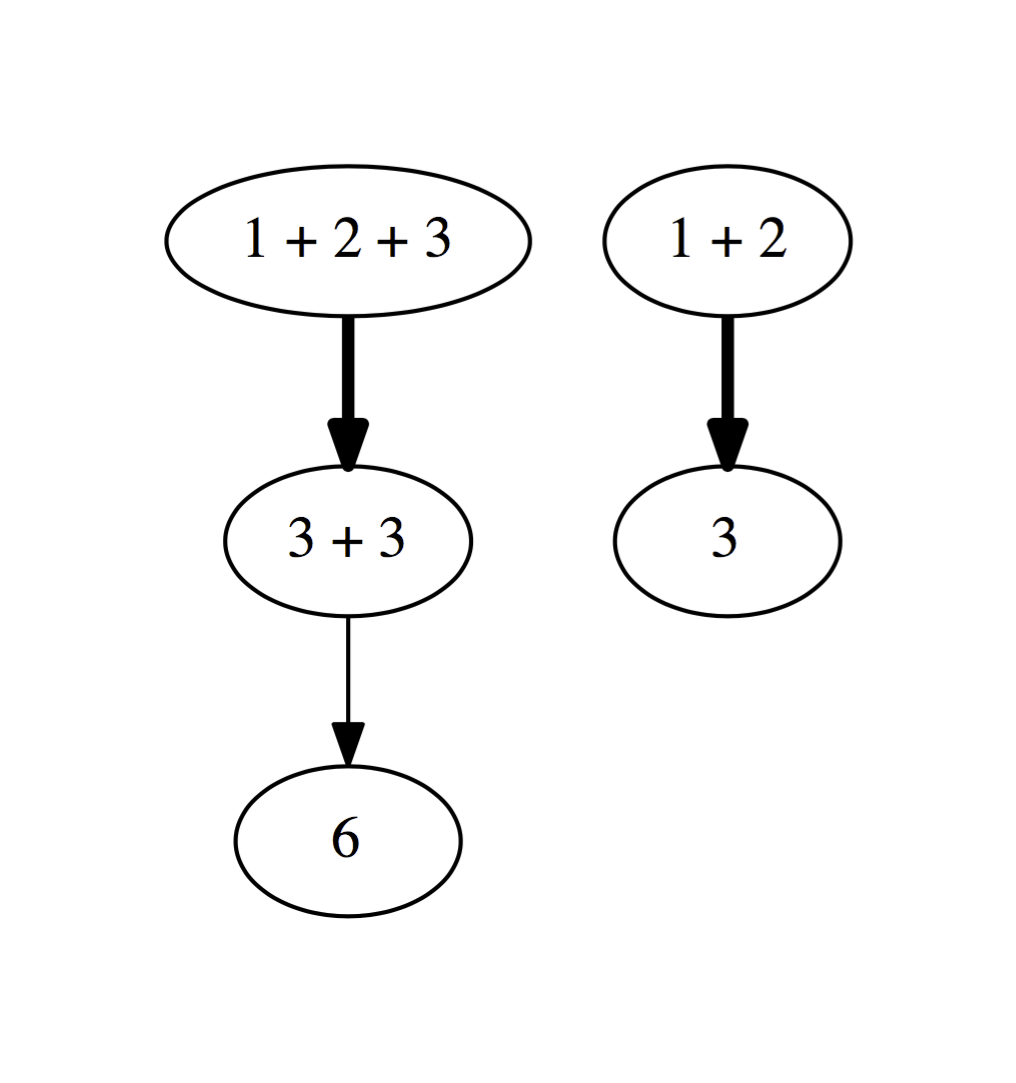
\includegraphics[height=2in]{nanomaly/simple.png}
  \caption{The reduction graph for \texttt{1+2+3}. The two edges
    produced by the transition from \texttt{1+2+3} to \hbox{\texttt{3+3}}
    are highlighted.}
\label{fig:simple-reduction-hi}
\end{figure}
%
Notice that when we transition from @1+2+3@ to @3+3@ we collect
both that edge \emph{and} an edge from the sub-term @1+2@ to @3@.
%
These additional edges allow us to implement two common debugging
operations \emph{post-hoc}: ``step into'' to zoom in on a specific
function call, and ``step over'' to skip over an uninteresting
sub-computation.

\paragraph{Interacting with the graph}
The reduction graph is useful for formulating and executing traversals,
but displaying it all at once would quickly become overwhelming.
%
Our interaction begins by displaying a big-step reduction, \ie the
witness followed by the stuck term.
%
The user can then progressively fill in the hidden steps of the
computation by selecting a visible term and choosing one of the
applicable traversal strategies --- described in
\S~\ref{sec:interactive} --- to insert another term into the
visualization.

\paragraph{Jump-compressed Witnesses}
It is rare for the initial state of the visualization to be
informative enough to diagnose the error.
%
Rather than abandon the user, we provide a short-cut to expand the witness
to a \emph{jump-compressed} trace, which contains every function call
and return step.
%
The jump-compressed trace abstracts the computation as a sequence of
call-response pairs, providing a high-level overview of steps taken
to reach the crash, and a high level of compression compared to the
full trace.
%
For example, the jump-compressed trace in Figure~\ref{fig:factorial}
contains 4 nodes compared to the 19 in the fully expanded trace.
%
Our benchmark suite of student programs shows that jump-compression is
practical, with an average jump-compressed trace size of 7 nodes and a
median of 5.

% A sample interaction with the trace of @fac 1@ can be seen in
% Figure~\ref{fig:nanomaly-factorial}.
% %
% % \begin{figure*}[t]
% % \centering
% % 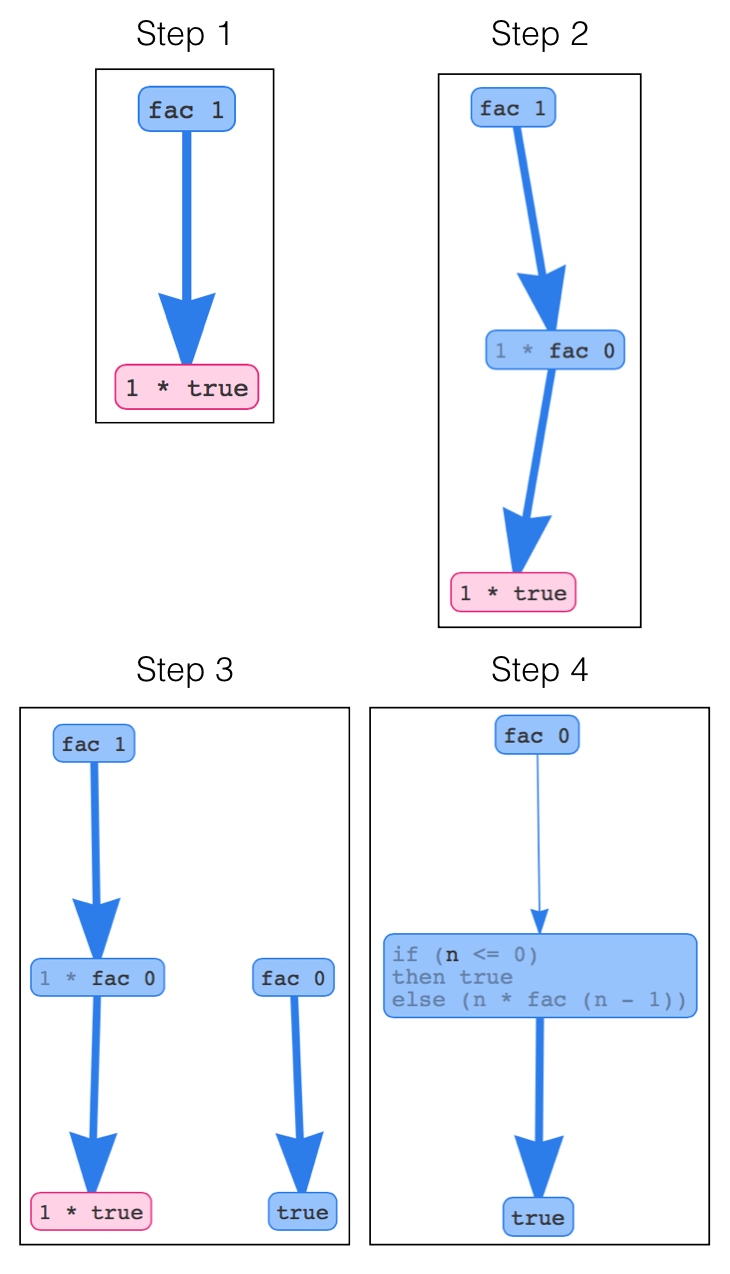
\includegraphics[width=0.8\linewidth]{fac-steps.png}
% % \caption{A sequence of interactions with the trace of
% %   \texttt{fac 1}. The stuck term is red, in each node the redex is
% %   highlighted. Thick arrows denote a multi-step transition, thin arrows
% %   denote a single-step transition. We start in step 1. In step 2 we jump
% %   forward from the witness to the next function call. In step 3 we step
% %   into the recursive \texttt{fac 0} call, which spawns a new ``thread''
% %   of execution. In step 4 we take a single step forward from
% %   \texttt{fac 0} (hiding the context for space).}
% % \label{fig:nanomaly-factorial}
% % \end{figure*}
% %
% The initial state of the visualization tells us that after some number
% of steps -- the thick arrow denotes a multi-step transition -- we try to
% multiply @1@ by @true@.

% Upon seeing the stuck term, we might wonder where @true@ came from.
% %
% To investigate we select the stuck term and click the ``jump backward''
% button to search backwards from the stuck term for the most recent
% function call, which brings us to @1 * fac 0@. Notice at this point that
% @fac 0@ is highlighted while @1 *@ is grayed out. This tells us that
% @fac 0@ is the redex in this term.

% @fac 0@ seems like the right thing to do so we choose to ``step into''
% it, which inserts a new multi-step transition from @fac 0@ to @true@.
% %
% Finally, we take a ``step forward'' from \hbox{@fac 0@,} bringing us to @fac@'s
% body. If we mouse over the body term we will see a popup with the
% environment at this point, notably telling us that @n = 0@. At this point
% it is clear that @fac@ handles the @n <= 0@ case incorrectly and should
% instead return an @int@.

% Upon seeing the stuck term, one might wonder where the @function@
% came from.
% %
% To investigate we select the stuck term and click the ``jump backward''
% button to search backwards from the stuck term for the most recent
% function call, which brings us to @listReverse [] = w@, in the same
% context as before.
% %
% Uncontent with the explanation so far, we ``step forward'' twice from
% the @listReverse []@ term, bringing us to @helper [] = w@.
% %
% At this point it is clear that the @helper@ function is not defined
% correctly, we have supplied it with the single argument we expected and
% yet it still returned a @function@.

% The problem is that the @function@ keyword in \ocaml defines an
% anonymous function that takes a single argument and immediately does a
% case-analysis without giving the argument a name.
% %
% The solution is to replace @function@ with an explicit @match xs with@
% -- naming the value we wish to case-analyse.
% %
% After applying our fix, \nanomaly -- and more importantly \ocaml --
% decide that @listReverse@ is safe to run.
% \ES{these last few paragraphs probably belong in the overview}
%





%%% Local Variables:
%%% mode: latex
%%% TeX-master: "main"
%%% End:

\section{A Framework for Type Targeted Testing}\label{sec:framework}

Next, we describe a framework for type targeted testing, by formalizing
an abstract representation of refinement types~(\S~\ref{sec:reftypes}), 
describing the operations needed to generate tests from types~(\S~\ref{sec:targetable}), 
and then using the above to implement \toolname via a query-decode-check 
loop~(\S~\ref{sec:loop}). 
%
Subsequently, we instantiate the framework to obtain tests
for refined primitive types, lists, algebraic datatypes and higher-order 
functions~(\S~\ref{sec:list}).

%% Next, we describe an (abstract) representation of refinement types,
%% and show how to use them to implement the @query@, @decode@ and @check@ 
%% steps from Figure~\ref{fig:arch}.
 
\subsection{Refinement Types}\label{sec:reftypes}

\begin{figure}[t!]
\begin{mdframed}
\begin{CenteredBox}
\begin{code}
-- Manipulating Refinements
refinement :: RefType -> Refinement
subst      :: RefType -> [(Var, Var)] -> RefType

-- Manipulating Types
unfold     :: Ctor  -> RefType -> [(Var, RefType)]
binder     :: RefType -> Var
proxy      :: RefType -> Proxy a 
\end{code}
\end{CenteredBox}
\end{mdframed}
\caption{Refinement Type API}\label{fig:rtype}
\end{figure}

A refinement type is a type, where each component is 
decorated with a predicate from a refinement logic. 
%
For clarity, we describe refinement types and refinements 
abstractly as @RefType@ and @Refinement@ respectively.
%
We write @Var@ as an alias for @Refinement@ that is 
typically used to represent logical variables appearing
within the refinement.

\mypara{Notation} 
In the sequel, we will use % backticks
double brackets $\meta{}$ to represent the 
various entities in the meta-language used to describe \toolname. 
%
For example, 
|$\meta{k}$|,
|$\meta{k \leq len\ v}$|, and
|$\meta{\reft{v}{[Score]}{k \leq len\ v}}$|
% \hbox{@`{v:[Score] | x0 <= len v}`@}
are the @Var@, @Refinement@, and @RefType@
representing the corresponding entities written in the brackets.


Next, we describe the various operations over them 
needed to implement \toolname.
These operations, summarized in Figure~\ref{fig:rtype}, 
fall into two categories: those which manipulate the 
\emph{refinements} and those which manipulate the 
\emph{types}.

\mypara{Operating on Refinements} 
To generate constraints and check inhabitation, we use 
the function @refinement@ which returns the (top-level) refinement
that decorates the given refinement type.
%
We will generate fresh @Var@s to name values of components, and will 
use @subst@ to replace the free occurrences of variables in a given \hbox{@RefType@.}
%
Suppose that @t@ is the @RefType@ represented by
\hbox{|$\meta{\reft{v}{[Score]}{k \leq len\ v}}$|.} Then,
%
\begin{itemize}
\item{@refinement t@} evaluates to |$\meta{k \leq len\ v}$| and
\item{|subst t [($\meta{k}$, $\meta{x_0}$)]|} evaluates to |$\meta{\reft{v}{[Score]}{x_0 \leq len\ v}}$|.
\end{itemize}

\mypara{Operating on Types} 
To build up compound values (\eg lists) from components 
(\eg an integer and a list), 
%
@unfold@ breaks a @RefType@ (\eg a list of integers) into its 
constituents (\eg an integer and a list of integers) at a given 
constructor (\eg ``cons'').
%
@binder@ simply extracts the @Var@ representing the
value being refined from the \hbox{@RefType@.}
%
To write generic functions over @RefType@s and use Haskell's
type class machinery to @query@ and @decode@ components of
types, we associate with each refinement type a \emph{proxy}
representing the corresponding Haskell type (in practice
this must be passed around as a separate argument).
%
For example, if @t@ is \hbox{|$\meta{\reft{v}{[Score]}{k \leq len\ v}}$|,} 
%
\begin{itemize}
\item{|unfold $\meta{:}$ t|} evaluates to |[($\meta{x}$, $\meta{Score}$), ($\meta{xs}$, $\meta{[Score]}$)]|,
\item{@binder t@} evaluates to |$\meta{v}$|, and
\item{@proxy t@} evaluates to a value of type @Proxy [Int]@.
\end{itemize}

\subsection{The \texttt{Targetable} Type Class}\label{sec:targetable}

% query  :: Haskell-Logic -> Gen SMT-Logic
% decode :: SMT-Value     -> Haskell-Value
% encode :: Haskell-Value -> SMT-Logic 

Following \quickcheck, we encapsulate the key operations needed
for type-targeted testing in a type class @Targetable@ 
(Figure~\ref{fig:targetable}). 
%
\begin{figure}
\begin{mdframed}
\begin{CenteredBox}
\begin{code}
class Targetable a where
  query  :: Proxy a -> Int -> RefType -> SMT Var
  decode :: Var -> SMT a
  check  :: a -> RefType -> SMT (Bool, Var)
  toReft :: a -> Refinement
\end{code}
\end{CenteredBox}
\end{mdframed}
\caption{The class of types that can be tested by \toolname}\label{fig:targetable}
\end{figure}
%
This class characterizes the set of types which can be tested 
by \toolname. All of the operations can interact with an external SMT 
solver, and so return values in an @SMT@ monad.

\begin{itemize}
\item{@query@} takes a \emph{proxy} for the Haskell type
   for which we are generating values, an integer 
   \emph{depth} bound, and a \emph{refinement type}
   describing the desired constraints, and generates a set of 
   logical constraints and a @Var@ that represents the 
   constrained value.

\item{@decode@} takes a @Var@, generated via a previous 
   @query@ and queries the model returned by the SMT solver
   to construct a Haskell value of type @a@.
 
\item{@check@} takes a value of type @a@, translates 
   it back into logical form, and verifies that it inhabits
   the output type @t@.
   
\item{@toReft@} takes a value of type @a@ and translates it
   back into logical form (a specialization of @check@).
\end{itemize}

\subsection{The Query-Decode-Check Loop}\label{sec:loop}



Figure~\ref{fig:arch} summarizes the overall implementation of 
\toolname, which takes as input a function @f@ and its refinement 
type specification @t@ and proceeds to test the function against 
the specification via a \emph{query-decode-check} loop:
%
(1) First, we translate the refined @inputTypes@ into a logical \emph{query}.
%
(2) Next, we \emph{decode} the model (\ie satisfying assignment) for the 
    query returned by the SMT solver to obtain concrete @inputs@.
%
(3) Finally, we @execute@ the function @f@ on the @inputs@ to get the 
    corresponding @output@, which we @check@ belongs to the specified 
    @outputType@. If the @check@ fails, we return the @inputs@ as a counterexample.
%
After each test, \toolname, refutes the given test to force the SMT 
solver to return a different set of inputs, and this process is repeated until 
a user specified number of iterations. The @checkSMT@ call may fail
to find a model meaning that we have exhaustively tested all inputs upto
a given @testDepth@ bound. If all iterations succeed, \ie no counterexamples
are found, then \toolname returns @Ok@, indicating that @f@ satisfies @t@ 
up to the given depth bound.

\begin{figure}[ht!]
\begin{mdframed}
\begin{CenteredBox}
\begin{code} 
target f t = do 
  let txs = inputTypes t
  vars  <- forM txs $ \tx -> 
             query (proxy tx) testDepth tx -- Query
  forM [1 .. testNum] $ \_ -> do
    hasModel <- checkSMT 
    when hasModel $ do
      inputs <- forM vars decode           -- Decode
      output <- execute f inputs                        
      let su = zip (map binder txs) (map toReft inputs)
      let to = outputType t `subst` su
      (ok,_) <- check output to            -- Check
      if ok then 
        refuteSMT 
      else 
        throw (CounterExample inputs)     
  return Ok
\end{code}
\end{CenteredBox}
\end{mdframed}
\caption{Implementing \toolname via a \emph{query-decode-check} loop}\label{fig:arch}
\end{figure}

\section{Instantiating the \toolname Framework}\label{sec:list}

Next, we describe a concrete instantiation of \toolname for lists.
%
We start with a constraint generation API~(\S~\ref{sec:constraint}). 
%
Then we use the API to implement the key operations 
\hbox{@query@~(\S~\ref{sec:query}),} 
\hbox{@decode@~(\S~\ref{sec:decode}),} 
\hbox{@check@~(\S~\ref{sec:check}),} and
\hbox{@refuteSMT@~(\S~\ref{sec:refute}),} 
thereby enabling \toolname to automatically test functions over lists.
We omit the definition of @toReft@ as it follows directly from the
definition of @check@.
%
Finally, we show how the list instance can be generalized to algebraic 
datatypes and higher-order functions~(\S~\ref{sec:generic}).

\subsection{SMT Solver Interface}\label{sec:constraint}

Figure~\ref{fig:smt} describes the interface to the SMT 
solvers that \toolname uses for constraint generation and 
model decoding. The interface has functions to 
%
(a)~generate logical variables of type @Var@, 
%
(b)~constrain their values using @Refinement@ predicates, and
%
(c)~determine the values assigned to the variables in satisfying models.

\begin{figure}[ht!]
\begin{mdframed}
\begin{CenteredBox}
\begin{code} 
fresh     :: SMT Var
guard     :: Var -> SMT a      -> SMT a 
constrain :: Var -> Refinement -> SMT ()

apply     :: Ctor -> [Var] -> SMT Var 
unapply   :: Var  -> SMT (Ctor, [Var])

oneOf     :: Var -> [(Var, Var)] -> SMT ()
whichOf   :: Var -> SMT Var

eval      :: Refinement -> SMT Bool
\end{code}
\end{CenteredBox}
\end{mdframed}
\caption{SMT Solver API}\label{fig:smt}
\end{figure}

\begin{itemize}

\item{@fresh@} allocates a new logical variable.

\item{@guard b act@} ensures that all the constraints 
generated by @act@ are \emph{guarded by} the choice 
variable @b@. That is, if @act@ generates the constraint 
$p$ then @guard b act@ generates the (implication) 
constraint ${b \Rightarrow p}$.

\item{@constrain x r@} generates a constraint that @x@ 
satisfies the refinement predicate @r@.

\item{@apply c xs@} generates a new @Var@ for the folded up value 
obtained by applying the constructor @c@ to the fields @xs@,
while also generating constraints from the measures. For example, 
{|apply $\meta{:}$ [$\meta{x_1}$, $\meta{xs_1}$]|} returns |$\meta{\lcons{\cvar{x}_1}{\cvar{xs}_1}}$|
%%%% \ES{$\lcons{\cvar{x}_1}{\cvar{xs}_1}$ doesn't look like a Var.. 
%%%% I guess this works since we've said that Var = Refinement, and 
%%%% it \emph{should} end up generating the constraints from the 
%%%% overview, but still.. I think we could easily confuse people 
%%%% here because of preconceived notions of what a Var is.}
and generates the constraint
${\clen{(\lcons{\cvar{x}_1}{\cvar{xs}_1})} = 1 + \clen{\cvar{xs}_1}}$.

\item{@unapply x@} returns the @Ctor@ and @Var@s from which the input 
@x@ was constructed. 

\item{@oneOf x cxs@} generates a constraint that @x@ equals exactly
one of the elements of @cxs@. For example, 
{|oneOf $\meta{xs_0}$ [($\meta{c_{00}}$,$\meta{[]}$),($\meta{c_{01}}$,$\meta{x_1 : xs_1}$)]|} 
yields:
$$(\cvar{c}_{00} \Rightarrow \cvar{xs}_0 = \lnil) \wedge 
  (\cvar{c}_{01} \Rightarrow \cvar{xs}_0 = \lcons{\cvar{x}_1}{\cvar{xs}_1}) \wedge 
  (\cvar{c}_{00} \oplus \cvar{c}_{01})$$

\item{@whichOf x@} returns the particular alternative that was 
assigned to @x@ in the current model returned by the 
SMT solver. Continuing the previous example, if the model sets 
|$\meta{c_{00}}$| (resp. |$\meta{c_{01}}$|) to $\ttrue$, |whichOf $\meta{xs_0}$| returns 
|$\meta{[]}$| (resp \hbox{|$\meta{x_1 : xs_1}$|).}

\item{@eval r@} checks the validity of a refinement with no free variables. For
  example, |eval $\meta{len\ (1 : []) > 0}$| would return @True@.

\end{itemize}

\subsection{Query}\label{sec:query}

Figure~\ref{fig:query} shows the procedure for constructing a 
@query@ from a refined list type, \eg the one required as an input 
to the @best@ or @insert@ functions from \S~\ref{sec:overview}.

\begin{figure}[t!]
\begin{mdframed}
\begin{CenteredBox}
\begin{mcode}
query p d t = do
  let cs = ctors d
  bs <- forM cs (\_ -> fresh)
  xs <- zipWithM (queryCtor (d-1) t) bs cs
  x  <- fresh 
  oneOf x     (zip bs xs)
  constrain x (refinement t)
  return x

queryCtor d t b c = guard b (do
  let fts = unfold c t
  fs'    <- scanM (queryField d) [] fts
  x      <- apply c fs'
  return x)

queryField d su (f, t) = do
  f' <- query (proxy t) d (t `subst` su)
  return ((f, f') : su, f')                    
ctors d
  | d > 0     = [ $\meta{:}$, $\meta{[]}$ ]
  | otherwise = [ $\meta{[]}$ ]
\end{mcode}
\end{CenteredBox}
\end{mdframed}
\caption{Generating a Query}\label{fig:query}
\end{figure}
% queryField :: Int -> Subst -> (Var, RefType) -> Gen (Subst, Var) 
% queryCtor :: Int -> RefType -> Choice -> Ctor -> Gen Var





\mypara{Lists}
@query@ returns a @Var@ that represent \emph{all} lists up to 
depth @d@ that satisfy the logical constraints associated with 
the refined list type @t@.
%
To this end, it invokes @ctors@ to obtain all of the suitable
constructors for depth @d@. For lists, when
the depth is @0@ we should only use the |$\meta{[]}$| constructor,
otherwise we can use either |$\meta{:}$| or |$\meta{[]}$|. 
This ensures that @query@ terminates after encoding all possible
lists up to a given depth \hbox{@d@.}
%
Next, it uses @fresh@ to generate a distinct \emph{choice} 
variable for each constructor, and calls \hbox{@queryCtor@ to}
generate constraints and a corresponding symbolic @Var@ 
for each constructor. 
%
The choice variable for each constructor is supplied to 
@queryCtor@ to ensure that the constraints are \emph{guarded}, 
\ie only required to hold \emph{if} the corresponding choice 
variable is selected in the model and not otherwise.
%
Finally, a fresh @x@ represents the value at depth @d@ and 
is constrained to be @oneOf@ the alternatives represented 
by the constructors, and to satisfy the top-level refinement of @t@.
%
% Note that the refinements of the components of @t@ will have already 
% been used to constrain the individual alternatives @xs@.


\mypara{Constructors}
@queryCtor@ takes as input the refined list type @t@, 
a depth @d@, a particular constructor @c@ for the list 
type, and generates a query describing the \emph{unfolding}
of @t@ at the constructor @c@, guarded by the choice 
variable @b@ that determines whether this alternative 
is indeed part of the value.
%
These constraints are the conjunction of
those describing the values of the individual fields 
which can be combined via @c@ to obtain a @t@ value.
%
To do so, @queryCtor@ first @unfold@s the type @t@ at 
@c@, obtaining a list of constituent fields and their
respective refinement types @fts@. Next, it uses 
%
\begin{code}
  scanM :: Monad m => (a -> b -> m (a, c)) -> a -> [b] -> m [c]
\end{code}
%
to traverse the fields from left to right, building up 
representations of values for the fields from their 
unfolded refinement types.
%
Finally, we invoke @apply@ on @c@ and the fields @fs'@ to 
return a symbolic representation of the constructed value 
that is constrained to satisfy the measure properties of @c@.

\mypara{Fields}
@queryField@ generates the actual constraints for a
single field @f@ with refinement type @t@, by invoking
@query@ on @t@.  
%
The @proxy@ enables us to resolve the appropriate 
type-class instance for generating the query for 
the field's value.
%
Each field is described by a new symbolic name @f'@ which is 
@subst@ituted for the formal name of the field @f@ in the
refinements of subsequent fields, thereby tracking dependencies
between the fields.
%
For example, these substitutions ensure the values in 
the tail are greater than the head as needed by 
@OrdList@ from \S~\ref{sec:overview}.

\subsection{Decode}\label{sec:decode}
%
\begin{figure}[t!]
\begin{mdframed}
\begin{minipage}{0.45\textwidth}
\begin{CenteredBox}
\begin{code}
decode x = do 
  x'      <- whichOf x
  (c,fs') <- unapply x'
  decodeCtor c fs'
\end{code}
\end{CenteredBox}
\end{minipage}
%
\begin{minipage}{0.55\textwidth}
\begin{CenteredBox}
\begin{mcode}
decodeCtor $\meta{[]}$ []    = return []
decodeCtor $\meta{:}$ [x,xs] = do
  v  <- decode x
  vs <- decode xs
  return (v:vs)
\end{mcode}
\end{CenteredBox}
\end{minipage}
\end{mdframed}
\caption{Decoding Models into Haskell Values}\label{fig:decode}
\end{figure}
%
Once we have generated the constraints we query the SMT solver 
for a model, and if one is found we must \emph{decode} it into
a concrete Haskell value with which to test the given function.
Figure~\ref{fig:decode} shows how to decode an SMT model for lists. 

\mypara{Lists} @decode@ takes as input the top-level symbolic
representation @x@ and queries the model to determine which
alternative was assigned by the solver to @x@, \ie a nil or a cons.
Once the alternative is determined, we use @unapply@ to destruct 
it into its constructor @c@ and fields @fs'@, which are recursively
decoded by @decodeCtor@.

\mypara{Constructors} @decodeCtor@ takes the constructor @c@ and
a list of symbolic representations for fields, and decodes each 
field into a value and applies the constructor to obtain the 
Haskell value.
%
For example, in the case of the |$\meta{[]}$| constructor, there are no
fields, so we return the empty list. In the case of the |$\meta{:}$| 
constructor, we decode the head and the tail, and cons them to 
return the decoded value. 
%
@decodeCtor@ has the type
%
\begin{code}  
  Targetable a => Ctor -> [Var] -> SMT [a]
\end{code}
%
\ie if @a@ is a decodable type, then @decodeCtor@ suffices to decode lists of @a@.
%
Primitives like integers that are directly encoded 
in the refinement logic are the base case -- \ie the 
value in the model is directly translated into the 
corresponding Haskell value.


\subsection{Check}\label{sec:encode}\label{sec:check}
%
\begin{figure}[t!]
\begin{mdframed}
\begin{CenteredBox}
\begin{mcode}
check v t = do
  let (c,vs) = splitCtor v
  let fts    = unfold c t
  (bs, vs') <- fmap unzip (scanM checkField [] (zip vs fts))
  v'        <- apply c vs'
  let t'     = t `subst` [(binder t, v')]
  b'        <- eval (refinement t')
  return (and (b:bs), v')
  
checkField su (v, (f, t)) = do
  (b, v') <- check v (t `subst` su)
  return ((f, v') : su, (b, v'))

splitCtor []     = ($\meta{[]}$, [])
splitCtor (x:xs) = ($\meta{:}$, [x,xs])
\end{mcode}
\end{CenteredBox}
\end{mdframed}
\caption{Checking Outputs}\label{fig:check}
\end{figure}
%
The third step of the query-decode-check loop is to verify
that the output produced by the function under test indeed
satisfies the output refinement type of the function.
%
We accomplish this by \emph{encoding} the output value as a
logical expression, and evaluating the output refinement
applied to the logical representation of the output value.

@check@, shown in Figure~\ref{fig:check}, takes a Haskell
(output) value @v@ and the (output) refinement type @t@, and
recursively verifies each component of the output type. It
converts each component into a logical representation,
@subst@itutes the logical expression for the symbolic value,
and @eval@uates the resulting @Refinement@.

%% We accomplish this by \emph{encoding} the output value as a 
%% set of of logical constraints, and then querying the SMT 
%% solver to check consistency with the output type.

%% @check@, shown in Figure~\ref{fig:check}, takes a Haskell
%% (output) value @v@ and the (output) refinement type @t@,
%% converts @v@ into a logical representation while adding the
%% constraints imposed by @t@, and then checks the consistency
%% of the resulting constraint system.
%% %
%% @encode@ recursively translates the Haskell value into a set
%% of logical constraints, by unfolding the type @t@ to obtain
%% the types of the value's compenents, encoding the components
%% to obtain symbolic fields, invoking @apply@ on the fields to
%% assert the measure properties of the constructor, and
%% finally constraining the resulting symbolic value to satisfy
%% @t@'s refinement.

\subsection{Refuting Models} \label{sec:refute}

Finally, \toolname invokes @refuteSMT@ to \emph{refute} a 
given model in order to force the SMT solver to produce a 
different model that will yield a different test input.
%
A na\"{\i}ve implementation of refutation is as follows.
%
Let $X$ be the set of all variables appearing in the constraints.
%
Suppose that in the current model, each variable $x$ is assigned 
the value $\val{x}$.
%
Then, to refute the model, we add a \emph{refutation constraint} 
$
\vee_{x \in X} x \not = \val{x}
$.
That is, we stipulate that \emph{some} variable be assigned a 
different value.

The na\"{\i}ve  implementation is extremely inefficient.
The SMT solver is free to pick a different value for some 
\emph{irrelevant} variable which was not even used for decoding.
%
As a result, the next model can, after decoding, yield the 
\emph{same} Haskell value, thereby blowing up the number of 
iterations needed to generate all tests of a given size.

\toolname solves this problem by forcing the SMT solver to return
models that yield \emph{different decoded tests} in each iteration.
To this end \toolname restricts the refutation constraint to 
the set of variables that were actually used to @decode@ the 
Haskell value.
%
We track this set by instrumenting the @SMT@ monad to log the 
set of variables and choice-variables that are transitively 
queried via the recursive calls to @decode@.
%
That is, each call to @decode@ logs its argument, and each call 
to @whichOf@ logs the choice variable corresponding to the 
alternative that was returned.
%
Let $R$ be the resulting set of \emph{decode-relevant} variables.
\toolname refutes the model by using a \emph{relevant refutation constraint}
$
\vee_{x \in R} x \not = \val{x}
$
which ensures that the next model decodes to a different value.% than all preceding ones.


\subsection{Generalizing \toolname To Other Types}\label{sec:generic}

The implementation in \S~\ref{sec:list} is for % refined 
List types, but @ctors@, @decodeCtor@, and @splitCtor@ are the only 
functions that are List-specific. 
%
Thus, we can easily generalize the implementation to:
%
\begin{itemize}
%
\item{\emph{primitive datatypes}}, \eg integers, by returning an empty 
    list of constructors,
%    
\item{\emph{algebraic datatypes}}, by implementing @ctors@, @decodeCtor@, and @splitCtor@ for that type.
%
\item{\emph{higher-order functions}}, by lifting instances of @a@ to functions returning @a@.
\end{itemize}

\mypara{Algebraic Datatypes}
% 
Our List implementation has three pieces of type-specific logic:
%
\begin{itemize}
\item{@ctors@}, which returns a list of constructors to unfold;
%
\item{@decodeCtor@}, which decodes a specific @Ctor@; and
%
\item{@splitCtor@}, which splits a Haskell value into a pair of its @Ctor@ and fields. 
\end{itemize}

Thus, to instantiate \toolname on a new data type, all we need is to 
implement these three operations for the type. This implementation
essentially follows the concrete template for Lists.
In fact, we observe that the recipe is entirely mechanical boilerplate,  
and can be fully automated for \emph{all} algebraic data types by using 
a \emph{generics} library.

Any algebraic datatype (ADT) can be represented as a \emph{sum-of-products} 
of component types. A generics library, such as \GhcGenerics~\cite{magalhaes_generic_2010}, 
provides a \emph{univeral} sum-of-products type and functions to automatically 
convert any ADT to and from the universal representation.
Thus, to obtain @Targetable@ instances for \emph{any} ADT it suffices
to define a @Targetable@ instance for the \emph{universal} type.

Once the universal type is @Targetable@ we can automatically get an 
instance for any new user-defined ADT (that is an instance of @Generic@) as follows:
%
(1)~to generate a \emph{query} we simply create a query for 
    \GhcGenerics' universal representation of the refined type,
%
(2)~to \emph{decode} the results from the SMT solver, we 
    decode them into the universal representation and then use 
    \GhcGenerics to map them back into the user-defined type,
%
(3)~to \emph{check} that a given value inhabits a user-defined 
    refinement type, we check that the universal representation 
    of the value inhabits the type's universal counterpart.

The @Targetable@ instance for the universal representation is a 
generalized version of the List instance from \S~\ref{sec:list}, 
that relies on various technical details of \GhcGenerics.
% Thus, we defer it to
% \ifthenelse{\equal{\isTechReport}{true}}{Appendix~\ref{sec:genericapp}}{the Appendix}.

\mypara{Higher Order Functions} 
Our type-directed approach to specification makes it easy to extend
\toolname to higher-order functions. Concretely, it suffices to 
implement a type-class instance:
%
\begin{code}
  instance (Targetable input, Targetable output) 
    => Targetable (input -> output)
\end{code}
%
In essence, this instance uses the @Targetable@ 
instances for @input@ and @output@ to 
create an instance for functions from @input -> output@,
after which Haskell's type class machinery suffices to 
generate concrete function values.

To create such instances, we use the insight from 
\quickcheck, that to generate (constrained) functions,
we need only to generate \emph{output} values for the function. 
%
Following this route, we generate functions by creating 
new lambdas that take in the inputs from the calling context, 
and use their values to create queries for the output, after 
which we can call the SMT solver and decode the results 
to get concrete outputs that are returned by the lambda, 
completing the function definition. 
%
Note that we require @input@ to also be @Targetable@
so that we can encode the Haskell value in the refinement logic,
in order to constrain the output values suitably.
%
We additionally memoize the generated function to preserve the 
illusion of purity. 
%
It is also possible to, in the future, extend our 
implementation to refute functions by asserting 
that the output value for a given input be distinct 
from any previous outputs for that input.

\mysection{Evaluation}
\label{sec:nate:evaluation}
\pgfplotstableset{col sep=comma}

% \pgfplotstableread{nate/data/sp14/op+type+size/linear/results.csv}{\FeatureLinearBench}
% \pgfplotstablevertcat{\FeatureLinearBench}{nate/data/sp14/op+context+type+size/linear/results.csv}
% \pgfplotstablevertcat{\FeatureLinearBench}{nate/data/sp14/op+context-has+type+size/linear/results.csv}
% \pgfplotstablevertcat{\FeatureLinearBench}{nate/data/sp14/op+context-count+type+size/linear/results.csv}
% \pgfplotstableread{nate/data/sp14/op+type+size/hidden-10/results.csv}{\FeatureHiddenTBench}
% \pgfplotstablevertcat{\FeatureHiddenTBench}{nate/data/sp14/op+context+type+size/hidden-10/results.csv}
% \pgfplotstablevertcat{\FeatureHiddenTBench}{nate/data/sp14/op+context-has+type+size/hidden-10/results.csv}
% \pgfplotstablevertcat{\FeatureHiddenTBench}{nate/data/sp14/op+context-count+type+size/hidden-10/results.csv}
% \pgfplotstableread{nate/data/sp14/op+type+size/hidden-500/results.csv}{\FeatureHiddenFHBench}
% \pgfplotstablevertcat{\FeatureHiddenFHBench}{nate/data/sp14/op+context+type+size/hidden-500/results.csv}
% \pgfplotstablevertcat{\FeatureHiddenFHBench}{nate/data/sp14/op+context-has+type+size/hidden-500/results.csv}
% \pgfplotstablevertcat{\FeatureHiddenFHBench}{nate/data/sp14/op+context-count+type+size/hidden-500/results.csv}

% \pgfplotstableread{nate/data/sp14/op+type+size/hidden-10/results.csv}{\HiddenBench}
% \pgfplotstablevertcat{\HiddenBench}{nate/data/sp14/op+type+size/hidden-25/results.csv}
% \pgfplotstablevertcat{\HiddenBench}{nate/data/sp14/op+type+size/hidden-50/results.csv}
% \pgfplotstablevertcat{\HiddenBench}{nate/data/sp14/op+type+size/hidden-100/results.csv}
% \pgfplotstablevertcat{\HiddenBench}{nate/data/sp14/op+type+size/hidden-250/results.csv}
% \pgfplotstablevertcat{\HiddenBench}{nate/data/sp14/op+type+size/hidden-500/results.csv}
% % \pgfplotstablevertcat{\HiddenBench}{nate/data/sp14/op+context-count+type+size/hidden-10/results.csv}
% % \pgfplotstablevertcat{\HiddenBench}{nate/data/sp14/op+context-count+type+size/hidden-25/results.csv}
% % \pgfplotstablevertcat{\HiddenBench}{nate/data/sp14/op+context-count+type+size/hidden-50/results.csv}
% % \pgfplotstablevertcat{\HiddenBench}{nate/data/sp14/op+context-count+type+size/hidden-100/results.csv}
% % \pgfplotstablevertcat{\HiddenBench}{nate/data/sp14/op+context-count+type+size/hidden-250/results.csv}
% % \pgfplotstablevertcat{\HiddenBench}{nate/data/sp14/op+context-count+type+size/hidden-500/results.csv}

\pgfplotstableread{nate/data/sp14/baseline.csv}{\SpringBench}
\pgfplotstablevertcat{\SpringBench}{nate/data/sp14/ocaml/results.csv}
\pgfplotstablevertcat{\SpringBench}{nate/data/sp14/mycroft/results.csv}
\pgfplotstablevertcat{\SpringBench}{nate/data/sp14/sherrloc/results.csv}
\pgfplotstablevertcat{\SpringBench}{nate/data/sp14/op+context+type+size/linear/results.csv}
\pgfplotstablevertcat{\SpringBench}{nate/data/sp14/op+context+type+size/decision-tree/results.csv}
\pgfplotstablevertcat{\SpringBench}{nate/data/sp14/op+context+type+size/random-forest/results.csv}
\pgfplotstablevertcat{\SpringBench}{nate/data/sp14/op+context+type+size/hidden-10/results.csv}
\pgfplotstablevertcat{\SpringBench}{nate/data/sp14/op+context+type+size/hidden-500/results.csv}

\pgfplotstableread{nate/data/fa15/baseline.csv}{\FallBench}
\pgfplotstablevertcat{\FallBench}{nate/data/fa15/ocaml/results.csv}
\pgfplotstablevertcat{\FallBench}{nate/data/fa15/mycroft/results.csv}
\pgfplotstablevertcat{\FallBench}{nate/data/fa15/sherrloc/results.csv}
\pgfplotstablevertcat{\FallBench}{nate/data/fa15/op+context+type+size/linear/results.csv}
\pgfplotstablevertcat{\FallBench}{nate/data/fa15/op+context+type+size/decision-tree/results.csv}
\pgfplotstablevertcat{\FallBench}{nate/data/fa15/op+context+type+size/random-forest/results.csv}
\pgfplotstablevertcat{\FallBench}{nate/data/fa15/op+context+type+size/hidden-10/results.csv}
\pgfplotstablevertcat{\FallBench}{nate/data/fa15/op+context+type+size/hidden-500/results.csv}

\pgfplotstableread{nate/data/models/linear-op+slice-no-slice.cross.csv}{\SliceLinearBench}
\pgfplotstablevertcat{\SliceLinearBench}{nate/data/models/linear-op+slice.cross.csv}
\pgfplotstablevertcat{\SliceLinearBench}{nate/data/models/linear-op+slice-only-slice.cross.csv}
\pgfplotstableread{nate/data/models/hidden-500-op+slice-no-slice.cross.csv}{\SliceHiddenBench}
\pgfplotstablevertcat{\SliceHiddenBench}{nate/data/models/hidden-500-op+slice.cross.csv}
\pgfplotstablevertcat{\SliceHiddenBench}{nate/data/models/hidden-500-op+slice-only-slice.cross.csv}
% \pgfplotstablecreatecol[create col/assign/.code={%
%     \edef\entry{\thisrow{features}/\thisrow{model}}
%     \pgfkeyslet{/pgfplots/table/create col/next content}\entry
%   }]{tool}{\SliceBench}

\pgfplotstableread{nate/data/models/linear-op.cross.csv}{\FeatureLinearBench}
\pgfplotstablevertcat{\FeatureLinearBench}{nate/data/models/linear-op+size.cross.csv}
\pgfplotstablevertcat{\FeatureLinearBench}{nate/data/models/linear-op+context.cross.csv}
\pgfplotstablevertcat{\FeatureLinearBench}{nate/data/models/linear-op+type.cross.csv}
\pgfplotstablevertcat{\FeatureLinearBench}{nate/data/models/linear-op+context+size.cross.csv}
\pgfplotstablevertcat{\FeatureLinearBench}{nate/data/models/linear-op+type+size.cross.csv}
\pgfplotstablevertcat{\FeatureLinearBench}{nate/data/models/linear-op+context+type.cross.csv}
\pgfplotstablevertcat{\FeatureLinearBench}{nate/data/models/linear-op+context+type+size.cross.csv}
\pgfplotstableread{nate/data/models/linear-op.cross.csv}{\FeatureHiddenBench}
\pgfplotstablevertcat{\FeatureHiddenBench}{nate/data/models/hidden-500-op+size.cross.csv}
\pgfplotstablevertcat{\FeatureHiddenBench}{nate/data/models/hidden-500-op+context.cross.csv}
\pgfplotstablevertcat{\FeatureHiddenBench}{nate/data/models/hidden-500-op+type.cross.csv}
\pgfplotstablevertcat{\FeatureHiddenBench}{nate/data/models/hidden-500-op+context+size.cross.csv}
\pgfplotstablevertcat{\FeatureHiddenBench}{nate/data/models/hidden-500-op+type+size.cross.csv}
\pgfplotstablevertcat{\FeatureHiddenBench}{nate/data/models/hidden-500-op+context+type.cross.csv}
\pgfplotstablevertcat{\FeatureHiddenBench}{nate/data/models/hidden-500-op+context+type+size.cross.csv}
% \pgfplotstablecreatecol[create col/assign/.code={%
%     \edef\entry{\thisrow{features}/\thisrow{model}}
%     \pgfkeyslet{/pgfplots/table/create col/next content}\entry
%   }]{tool}{\FeatureBench}


We have implemented our technique for localizing type errors for a
purely functional subset of \ocaml with polymorphic types and functions.
%
We seek to answer four questions in our evaluation:
%
\begin{itemize}
\item \textbf{Blame Accuracy}
  %
  How often does \toolname
  blame a \emph{correct}
  location for the error?
  (\autoref{sec:nate:quantitative})
  %
  % We compare our technique with a variety of off-the-shelf classifiers
  % and find that our top-ranked blame assignments have an accuracy of
  % 72\%, compared to a state-of-the-art 56\%.
  % For how many ill-typed programs can we accurately predict the source
  % of the error?
\item \textbf{Feature Utility}
  %
  Which program \emph{features are required}
  to localize errors?
   (\autoref{sec:nate:feature-utility})
  % How much do the features described in \autoref{sec:nate:features}
  % contribute to our predictions?
\item \textbf{Interpretability}
  %
  %% Do the models learned by \toolname
  %% correspond to our intuition about
  %% the real causes of errors?
  Do the models match our intuition about type errors?
  (\autoref{sec:nate:qualitative})
\item \textbf{Blame Utility}
  Do \toolname's blame assignments help
  users diagnose type errors?
  (\autoref{sec:nate:user-study})
\end{itemize}
%
%\mypara{Summary of Results}
%
In the sequel we present our experimental
methodology \autoref{sec:nate:methodology} and
then drill into how we evaluated each of
the questions above.
%
However, for the impatient reader, we begin
with a quick summary of our main results:
%
%
%\begin{itemize}
%
%\item \textbf

\mypara{1. Data Beats Algorithms}
Our main result is that for type error
localization, data is indeed unreasonably
effective \citep{Halevy2009-so}.
%
When trained on student errors from one
instance of an undergraduate course and
tested on another instance,
\toolname's most sophisticated
\emph{neural network}-based
classifier's top-ranked
prediction blames the correct
sub-term \HiddenFhTopOne\% of the time
--- a good \ToolnameWinSherrloc points
higher than the state-of-the-art
\sherrloc's \SherrlocTopOne\%.
%
However, even \toolname's simple
\emph{logistic regression} based
classifier is correct \LinearTopOne\% of the time,
\ie \LinearWinSherrloc points better than \sherrloc.
%
When the top three predictions are considered,
\toolname is correct \HiddenFhTopThree\% of the time.

% \item \textbf
\mypara{2. Slicing Is Critical}
%
However, data is effective \emph{only}
when irrelevant sub-terms have been
sliced out of consideration.
%
In fact, perhaps our most surprising
result is that type error slicing and
local syntax alone yields
a classifier that is \SlicingWinOcaml points
better than \ocaml and on par with
\sherrloc.
%
That is, once we focus our classifiers on
slices, purely local syntactic features
perform as well as the
state-of-the-art.

%\item \textbf
\mypara{3. Size Doesn't Matter, Types Do}
%
We find that (after slices)
typing features
provide the biggest
improvement in accuracy.
%
Furthermore, we find contextual syntactic
features to be mostly (but not entirely)
redundant with typing features,
which supports the hypothesis that
the context's \emph{type} nicely
summarizes the properties of the
surrounding expressions.
%
Finally, we found that the \emph{size}
of the sub-expression was not very useful.
This was unexpected, as we thought
smaller expressions would be simpler, and
hence, more likely causes.

% \item \textbf
\mypara{4. Models Learn Typing Rules}
%
Finally, by investigating a few of the
predictions made by the \emph{decision tree}-based
models, we found that the models
appear to capture some simple and intuitive
rules for predicting well-typedness.
%
For example, if the left child of an application
is a function, then the application is likely
correct.

% in an application, if the
% left argument is a function then the
% error is likely on the right sub-term;
% in a function definition
% \RJ{fixme: orig
% defining a function is a fine thing
% to do?}
%
%\end{itemize}
% \RJ{eric please check the numbers -- we say 71, 72, 74, 91, 92, 94?}


\mysubsection{Methodology}
\label{sec:nate:methodology}
We answer our questions on the two datasets gathered in
\autoref{chp:data-collection}, which we will briefly describe
again.
% We answer our questions on two sets of data gathered from the
% undergraduate Programming Languages course at
% % \begin{anonsuppress}
% UC San Diego (IRB \#140608).
% \end{anonsuppress}
% \begin{noanonsuppress}
% AUTHOR's INSTITUTION.
% \end{noanonsuppress}
%
We recorded each interaction with the \ocaml top-level system while
students in our undergraduate Programming Languages course
worked on 23 programs from the first three homework
assignments, capturing ill-typed programs and, crucially, their
subsequent fixes.
%
The first dataset comes from the Spring 2014 class (\SPRING), with a
cohort of 46 students. The second comes from the Fall 2015 class
(\FALL), with a cohort of 56 students.
%
The extracted programs are relatively small, but they demonstrate a
range of functional programming idioms, \eg higher-order functions and
(polymorphic) algebraic data types.

\mypara{Feature Selection}
We extract 282 features from each sub-expression in a
program, including:
%
\begin{enumerate}
\item 45 local syntactic features. In addition to the syntax of \lang,
  we support the full range of arithmetic operators (integer and
  floating point), equality and comparison operators, character and
  string literals, and a user-defined % |expr| type of simple
  arithmetic
  expressions. We discuss the challenge of supporting other
  % user-defined
  types in \autoref{sec:nate:discussion}.
\item 180 contextual syntactic features. For each sub-expression we
  additionally extract the local syntactic features of its parent and
  first, second, and third (left-to-right) children. If an expression
  does not have a parent or children, these features will simply be
  disabled. If an expression has more than three children, the
  classifiers will receive no information about the additional
  children.
\item 55 typing features. In addition to the types of \lang, we support
  |int|s, |float|s, |char|s, |string|s, and the user-defined |expr|
  mentioned above. These features are extracted for each sub-expression
  and its context. % for the contextual sub-expressions.
\item One feature denoting the size of each sub-expression.
\item One feature denoting whether each sub-expression is part of the
  minimal type error slice. We use this feature as a ``hard''
  constraint, sub-expressions that are not part of the minimal slice
  will be preemptively discarded. We justify this decision in
  \autoref{sec:nate:feature-utility}.
\end{enumerate}

\mypara{Blame Oracle}
Recall from \autoref{sec:nate:labels} that we automatically extract a blame
oracle for each ill-typed program from the (AST) diff between it and the
student's eventual fix.
%
A disadvantage of using diffs in this manner is that students may have
made many, potentially unrelated, changes between compilations; at some
point the ``fix'' becomes a ``rewrite''.
%
We do not wish to consider the ``rewrites'' in our evaluation, so we
discard outliers where the fraction of expressions that have changed is
more than one standard deviation above the mean, establishing a diff
threshold of 40\%.
%
This accounts for roughly 14\% of each dataset, leaving us with
2,712 program pairs for \SPRING and 2,365 pairs for \FALL.

% we discard any program pairs where more than 40\%
% of the sub-expressions have changed.
% %
% We picked 40\% as an estimate of the inflection point where we could
% still retain the large majority of program pairs.
% % FIXME: Can you say that this dataset curation is similar to any other
% % datasets (e.g., the washington one)? Anything you could cite and discuss
% % here would take some of the pressure off.


\mypara{Accuracy Metric}
All of the tools we compare (with the exception of the standard \ocaml
compiler) can produce a list of potential error locations.
%
However, in a study of fault localization techniques,
\citet{Kochhar2016-oc} show that most developers will not consider more
than around five potential error locations before falling back to manual
debugging.
%
Type errors are relatively simple in comparison to general fault
localization, thus we limit our evaluation to the top three predictions
of each tool.
%
We evaluate each tool on whether a changed expression occurred in its
top one, top two, or top three predictions.

\mysubsection{Threats to Validity}
\label{sec:nate:validity}

Although our experiments demonstrate that our technique can pinpoint type
errors more accurately than the state of the art and that our features are
relevant to blame assignment, our results may not generalize.

One threat to validity associated with supervised machine learning is
overfitting (\ie learning a model that is too complex with respect to
the data).
%
A similar issue that arises in machine learning is model stability (\ie
can small changes to the training set produce large changes in the model?).
%
We mitigate these threats by:
%
(1) using separate training and testing datasets drawn from distinct
student populations (\autoref{sec:nate:quantitative}), demonstrating the
generality of our models; and
%
(2) via cross-validation on the joint dataset
(\autoref{sec:nate:feature-utility}), which demonstrates the stability of our
models by averaging the accuracy of 10 models trained on distinct
subsets of the data.

Our benchmarks were drawn from students in an undergraduate course and
may not be representative of other student populations.
%
We mitigate this threat by including the largest empirical evaluation of
type error localization that we are aware of: over 4,500 pairs of
ill-typed programs and fixes from two instances of the course, with
programs from 102 different students.
%
We acknowledge, of course, that students are not industrial programmers
and our results may not translate to large-scale software development;
however, we are particularly interested in aiding novice programmers
as they learn to work inside the type system.

A related threat to construct validity is our definition of the immedate
next well-typed program as the intended ground truth answer (see
\autoref{sec:nate:overview}, Challenge 2). Students may, in theory, submit
intermediate well-typed program ``rewrites'' between the original ill-typed
program and the final intended answer. Our approach to discarding outliers
(see \autoref{sec:nate:evaluation}) is designed to mitigate this threat.

Our removal of program pairs that changed too much, where our oracle
could not identify the blame of the other tools, or where the other
tools timed out or encountered unsupported language features is another
threat to validity.
%
It is possible that including the programs that changed excessively
would hurt our models, or that the other tools would perform
better on the programs with unsupported language features.
%
We note however that
%
(1) outlier removal is a standard technique in machine learning%
%\ES{CITE?}
; and
%
(2) our Top-1 accuracy margin is large enough that even if we assumed
that \sherrloc were perfect on all excluded programs,
% it would only tie our \hiddenFH. % in Top-1 accuracy.
we would still lead by 10 points.
%
%\ES{I think this is accurate, but should double check..}

Examining programs written in \ocaml as opposed to \haskell or any other
typed functional language poses yet another threat, common type errors
may differ in different languages.
%
\ocaml is, however, a standard target for research in type error
localization and thus our choice admits a direct comparison with prior
work.
%
Furthermore, the functional core of \ocaml that we support does not
differ significantly from the functional core of \haskell or SML, all of
which are effectively lambda calculi with a Hindley-Milner-style type
system.
% \footnote{\haskell's type classes are a notable exception, they
%   are also known to cause confusing type errors and would be interesting
%   to study as well.}

Finally, our use of student fixes as oracles
% for the source of type errors
assumes that students are able to correctly identify
the source of an error.
%
As the students are in the process of learning the language and type
system, this assumption may be faulty.
%
It may be that \emph{expert} users would disagree with many of the
student fixes, and that it is harder to learn a model of expert fixes,
or that the state of the art would be better at predicting expert fixes.
%
As we have noted before, we believe it is reasonable to use student
fixes as oracles because the student is the best judge of what she
\emph{intended}.


\mysubsection{Blame Accuracy}
\label{sec:nate:quantitative}

First, we compare the accuracy of our predictions to the
state of the art in type error localization.

\mypara{Baseline}
We provide two baselines for the comparison: a random choice of location
from the minimized type error slice, and the standard \ocaml compiler.

\mypara{State of the Art}
\mycroft~\citep{Loncaric2016-uk} localizes type errors by searching for
a minimal subset of typing constraints that can be removed, such that
the resulting system is satisfiable.
%
When multiple such subsets exist it can enumerate them, though it has no
notion of which subsets are \emph{more likely} to be correct, and thus
the order is arbitrary.
%
\sherrloc~\citep{Zhang2014-lv} localizes errors by searching the typing
constraint graph for constraints that participate in many unsatisfiable
paths and comparatively few satisfiable paths.
%
It can also enumerate multiple predictions, in descending order of
likelihood.

Comparing source locations from multiple tools with their own parsers is
not trivial.
%
Our experimental design gives the state of the art tools the ``benefit
of the doubt'' in two ways.
% To ensure a fair comparison when evaluating \mycroft and
% \sherrloc,
First, when evaluating \mycroft and \sherrloc, we did not consider
programs where they predicted locations that our oracle could not match
with a program expression: around 6\% of programs for \mycroft and 4\%
for \sherrloc.
%
Second, we similarly ignored programs where \mycroft or \sherrloc timed
out (after one minute) or where they encountered an unsupported language
feature: another 5\% for \mycroft and 12\% for \sherrloc.
%

\mypara{Our Classifiers}
We evaluate five classifiers, each trained on the full feature set.
% features: 44 local syntactic features, 176 contextual syntactic
% features, 55 typing features, and a single expression size feature.
% %
% \ES{should explain the make-up of these groups}
%
% We preemptively discard expressions that are not part of the minimal
% type error slice --- we will explain the rationale for this in
% \autoref{sec:nate:feature-utility} --- and thus the final feature count is
% 276.
%
These include:
%Our classifiers are:
%
\begin{description}
\item[\linear] A logistic regression trained with a learning rate
  $\eta = 0.001$, an $L_2$ regularization rate $\lambda = 0.001$, and a
  mini-batch size of 200.
\item[\dectree] A decision tree trained with the CART algorithm
  \citep{Breiman1984-qy} and an impurity threshold of $10^{-7}$ (used to
  avoid overfitting via early stopping).
\item[\forest] A random forest \citep{Breiman2001-wo} of 30
  estimators, with an impurity threshold of $10^{-7}$.
\item[\hiddenT and \hiddenFH] Two multi-layer perceptron neural
  networks, both trained with $\eta = 0.001$, $\lambda = 0.001$, and a
  mini-batch size of 200.
  %
  The first MLP contains a single hidden layer of 10 neurons, and the
  second contains a hidden layer of 500 neurons.
  %
  This gives us a measure of the complexity of the MLP's model, \ie
  if the model requires many compound features, one would expect \hiddenFH
  to outperform \hiddenT.
  % This allows us to investigate how well the MLP can \emph{compress} its
  % model (cf.~\cite{FIXME}).
  %
  The neurons use rectified linear units (ReLU) as their activation
  function, a common practice in modern neural networks.
\end{description}
%
All classifiers were trained for 20 epochs on one dataset
--- \ie they were shown each program 20 times ---
before being evaluated on the other.
%
The logistic regression and MLPs were trained with the \textsc{Adam}
optimizer \citep{Kingma2014-ng}, a variant of stochastic gradient
descent that has been found to converge faster.


% colors from http://colorbrewer2.org/?type=sequential&scheme=Blues&n=3
\definecolor{blue1}{HTML}{DEEBF7}
\definecolor{blue2}{HTML}{9ECAE1}
\definecolor{blue3}{HTML}{3182BD}
\definecolor{green1}{HTML}{E5F5E0}
\definecolor{green2}{HTML}{A1D99B}
\definecolor{green3}{HTML}{31A354}

% \begin{figure}[ht]
% \centering
% \begin{tikzpicture}
% \begin{axis}[
%   % ybar stacked,
%   width=12cm,
%   height=8cm,
%   title={Impact of Feature Set on Accuracy},
%   ylabel={Accuracy},
%   %ymin=0.2,
%   ymax=1,
%   yticklabel={\pgfmathparse{\tick*100}\pgfmathprintnumber{\pgfmathresult}\,\%},
%   ytick style={draw=none},
%   ymajorgrids = true,
%   symbolic x coords={op+type+size, op+context+type+size, op+context-has+type+size, op+context-count+type+size},
%   % enlarge x limits=0.25,
%   xtick=data,
%   xtick style={draw=none},
%   xticklabels={Type, Context-Is, Context-Has, Context-Count},
%   x tick label style={rotate=45},
%   reverse legend,
%   transpose legend,
%   legend style={legend pos = outer north east, legend columns=4},
% ]
% % \addplot[draw=black, fill=blue1] table[x=tool, y=top-1] {\HiddenBench};
% % \addplot[draw=black, fill=blue2] table[x=tool, y expr=\thisrow{top-2} - \thisrow{top-1}] {\HiddenBench};
% % \addplot[draw=black, fill=blue3] table[x=tool, y expr=\thisrow{top-3} - \thisrow{top-2}] {\HiddenBench};

% \addplot[mark options={fill=blue1, scale=1.5}, mark=square*]
%   table[x=features, y=top-1] {\FeatureHiddenFHBench};
% \addplot[mark options={fill=blue2, scale=1.5}, mark=square*]
%   table[x=features, y=top-2] {\FeatureHiddenFHBench};
% \addplot[mark options={fill=blue3, scale=1.5}, mark=square*]
%   table[x=features, y=top-3] {\FeatureHiddenFHBench};
% \addlegendentry{Top-1}
% \addlegendentry{Top-2}
% \addlegendentry{Top-3}
% \addlegendimage{empty legend}
% \addlegendentry{\hiddenFH}

% \addplot[mark options={fill=blue1, scale=1.5}, mark=*]
%   table[x=features, y=top-1] {\FeatureLinearBench};
% \addplot[mark options={fill=blue2, scale=1.5}, mark=*]
%   table[x=features, y=top-2] {\FeatureLinearBench};
% \addplot[mark options={fill=blue3, scale=1.5}, mark=*]
%   table[x=features, y=top-3] {\FeatureLinearBench};
% \addlegendentry{Top-1}
% \addlegendentry{Top-2}
% \addlegendentry{Top-3}
% \addlegendimage{empty legend}
% \addlegendentry{\linear}

% \end{axis}
% \end{tikzpicture}
% \caption{reuslts!}
% \label{fig:results}
% \end{figure}

% \begin{figure}[ht]
% \centering
% \begin{tikzpicture}
% \begin{axis}[
%   ybar stacked,
%   width=12cm,
%   height=8cm,
%   title={Impact of Hidden Layer Size on Accuracy},
%   ylabel={Accuracy},
%   bar width=20pt,
%   %ymin=0.2,
%   ymax=1,
%   yticklabel={\pgfmathparse{\tick*100}\pgfmathprintnumber{\pgfmathresult}\,\%},
%   ytick style={draw=none},
%   ymajorgrids = true,
%   symbolic x coords={op+type+size/hidden-10, op+type+size/hidden-25, op+type+size/hidden-50,
%                      op+type+size/hidden-100, op+type+size/hidden-250, op+type+size/hidden-500},
%   % enlarge x limits=0.25,
%   xtick=data,
%   xtick style={draw=none},
%   xticklabels={\hiddenT, \hiddenTF, \hiddenF, \hiddenH, \hiddenTHF, \hiddenFH},
%   x tick label style={rotate=45},
%   reverse legend,
%   legend style={legend pos = north west},
% ]
% \addplot[draw=black, fill=blue1] table[x=tool, y=top-1] {\HiddenBench};
% \addplot[draw=black, fill=blue2] table[x=tool, y expr=\thisrow{top-2} - \thisrow{top-1}] {\HiddenBench};
% \addplot[draw=black, fill=blue3] table[x=tool, y expr=\thisrow{top-3} - \thisrow{top-2}] {\HiddenBench};
% % \addplot[draw=black, fill=blue1] table[x=tool, y=top-1] {\HiddenBench};
% % \addplot[draw=black, fill=blue2] table[x=tool, y=top-2] {\HiddenBench};
% % \addplot[draw=black, fill=blue3] table[x=tool, y=top-3] {\HiddenBench};
% \legend{Top-1, Top-2, Top-3}
% \end{axis}
% \end{tikzpicture}
% \caption{reuslts!}
% \label{fig:results}
% \end{figure}

\begin{figure}[t]
\centering
\begin{tikzpicture}
\begin{axis}[
  ybar stacked,
  width=14cm,
  height=6cm,
  title={Accuracy of Type Error Localization Techniques},
  ylabel={Accuracy},
  bar width=0.5cm,
  ymin=0.2,
  ymax=1,
  ytick={0.2, 0.3, 0.4, 0.5, 0.6, 0.7, 0.8, 0.9, 1.0},
  yticklabel={\pgfmathparse{\tick*100}\pgfmathprintnumber{\pgfmathresult}\,\%},
  ytick style={draw=none},
  ymajorgrids = true,
  symbolic x coords={baseline, ocaml, mycroft, sherrloc,
                     op+context+type+size/linear,
                     op+context+type+size/decision-tree,
                     op+context+type+size/random-forest,
                     op+context+type+size/hidden-10,
                     op+context+type+size/hidden-500},
  %enlarge x limits=0.07,
  xtick=data,
  xtick style={draw=none},
  xticklabels={\random, \ocaml, \mycroft, \sherrloc,
               \linear, \dectree, \forest, \hiddenT, \hiddenFH},
  x tick label style={rotate=45, anchor=north east},
  %x tick label style={font=\small},
  y tick label style={font=\small},
  reverse legend,
  transpose legend,
  legend style={legend pos = north west, legend columns=4, font=\footnotesize},
]

% ES: NOTE: ORDER OF PLOTS/LEGEND ENTRIES MATTERS

\addplot[draw=black, fill=green1, bar shift=.25cm] table[x=tool, y=top-1] {\FallBench};
\addlegendentry{Top-1}
\addplot[draw=black, fill=green2, bar shift=.25cm] table[x=tool, y expr=\thisrow{top-2} - \thisrow{top-1}] {\FallBench};
\addlegendentry{Top-2}
\addplot[draw=black, fill=green3, bar shift=.25cm] table[x=tool, y expr=\thisrow{top-3} - \thisrow{top-2}] {\FallBench};
\addlegendentry{Top-3}
\addlegendimage{empty legend}
\addlegendentry{\FALL}

\resetstackedplots

\addplot[draw=black, fill=blue1, bar shift=-.25cm] table[x=tool, y=top-1] {\SpringBench};
\addlegendentry{Top-1}
\addplot[draw=black, fill=blue2, bar shift=-.25cm] table[x=tool, y expr=\thisrow{top-2} - \thisrow{top-1}] {\SpringBench};
\addlegendentry{Top-2}
\addplot[draw=black, fill=blue3, bar shift=-.25cm] table[x=tool, y expr=\thisrow{top-3} - \thisrow{top-2}] {\SpringBench};
\addlegendentry{Top-3}
\addlegendimage{empty legend}
\addlegendentry{\SPRING}


%\legend{Top-1, Top-2, Top-3}
\end{axis}
\end{tikzpicture}
\caption[Results of our comparison of type error localization
  techniques.]{
  %
  Results of our comparison of type error localization
  techniques.
  %
  We evaluate all techniques separately on two cohorts of
  students from different instances of an undergraduate
  Programming Languages course.
  %
  Our classifiers were trained on one cohort and evaluated on the other.
  %
  All of our classifiers outperform the state-of-the-art techniques
  \mycroft and \sherrloc.%  by a 10--15\% margin in Top-1 accuracy (with
%   the exception of \linear which is only slightly better than \sherrloc).
%
}
\label{fig:accuracy-results}
\end{figure}


\mypara{Results}
\autoref{fig:accuracy-results} shows the results of our experiment.
%
Localizing the type errors in our benchmarks amounted, on average, to
selecting one of 3 correct locations out of a slice of 10.
%
Our classifiers consistently outperform the competition, ranging from
\LinearTopOne\% Top-1 accuracy (\LinearTopThree\% Top-3)
for the \linear classifier to
\HiddenFhTopOne\% Top-1 accuracy (\HiddenFhTopThree\% Top-3)
for the \hiddenFH.\@
%
Our baseline of selecting at random achieves \BaselineTopOne\% Top-1
accuracy (\BaselineTopThree\% Top-3),
while \ocaml achieves a Top-1 accuracy of \OcamlTopOne\%.
%
Interestingly, one only needs two \emph{random} guesses to outperform
\ocaml, with \BaselineTopTwo\% accuracy.
%
\sherrloc outperforms both baselines, and comes close to our \linear classifier,
with \SherrlocTopOne\% Top-1 accuracy (\SherrlocTopThree\% Top 3),
while \mycroft underperforms \ocaml at \MycroftTopOne\% Top-1 accuracy.
%
% Finally, we find that \emph{all} of our classifiers outperform \sherrloc,
% ranging from 58--62\% Top-1 accuracy (86--88\% Top-3) for the \linear
% classifier to 71--74\% Top-1 accuracy (91\% Top-3) for the \hiddenFH.

Surprisingly, there is little variation in accuracy between our
classifiers.
%
With the exception of the \linear model, they all achieve around 70\%
Top-1 accuracy and around 90\% Top-3 accuracy.
%
This suggests that the model they learn is relatively simple.
%
In particular, notice that although the \hiddenT has $50\times$ \emph{fewer}
hidden neurons than the \hiddenFH, it only loses around 4\% accuracy.
% In particular, notice that the \hiddenT only loses around 2\% accuracy
% compared to the \hiddenFH,
%
We also note that our classifiers consistently perform better when
trained on the \FALL programs and tested on the \SPRING programs than
vice versa.
% , they appear to generalize better from the \FALL data.
% FIXME: Why? What is your explanation for this? Is it just sizes of those
% datasets or something qualitative about the program pairs in them?

\mysubsection{Feature Utility}
\label{sec:nate:feature-utility}
We have shown that we can train a classifier to effectively localize
type errors, but which of the feature classes from
\autoref{sec:nate:features} are contributing the most to our accuracy?
%
We focus specifically on feature \emph{classes} rather than individual
features as our 282 features are conceptually grouped into a much
smaller number of \emph{categorical} features.
%
For example, the syntactic class of an expression is conceptually a
feature but there are 45 possible values it could take; to encode this
feature for learning we split it into 45 distinct binary features.
%
Analyses that focus on individual features, \eg \textsc{ANOVA},
are difficult to interpret in our setting, as they will tell us the
importance of the binary features but not the higher-level categorical
features.
%
Thus, to answer our question we investigate the performance of
classifiers trained on various subsets of the feature classes.

\mysubsubsection{Type Error Slice}
\label{sec:nate:type-error-slice}
First we must justify our decision to automatically exclude expressions
outside the minimal type error slice from consideration.
%
% The \InSlice feature should be highly predictive --- a fix must change
% at least one expression in the type error slice.
% %
% Thus, our first experiment seeks to quantify the impact of \InSlice by
% comparing the accuracy of our classifiers on three sets of features:
%
Thus, we compare our classifiers on three sets of features:
%
\begin{enumerate}
\item A baseline with only local syntactic features and no
  preemptive filtering by \InSlice.
\item The features of (1) extended with \InSlice.
\item The same features as (1), but we preemptively discard samples
  where \InSlice is disabled.
\end{enumerate}
%
The key difference between (2) and (3) is that a classifier for (2) must
\emph{learn} that \InSlice is a strong predictor.
%
In contrast, a classifier for (3) must only learn about the syntactic
features, the decision to discard samples where \InSlice is disabled has
already been made by a human.
%
This has a few additional advantages: it reduces the set of candidate
locations by a factor of 7 on average, and it guarantees that any
prediction made by the classifier can fix the type error.
%
We expect that (2) will perform better than (1) as it contains more
information, and that (3) will perform better than (2) as the classifier
does not have to learn the importance of \InSlice.

% FIXME: Wes feels that there should be a sentence in the next mypara
% explaining to the reader why we didn't just use an ANOVA or the ReliefF
% method or whatever to figure out feature importance. Feature overlap?

We tested our hypothesis with the \linear and
%
\hiddenFH\footnote{A layer of 500 neurons is excessive when we have so few
  input features --- we use \hiddenFH for continuity with the
  surrounding sections.}
%
classifiers, cross-validated ($k=10$) over the combined SP14/FA15
dataset.
% We used a learning rate $\eta=0.001$, $L_2$ regularization rate
%$\lambda=0.001$, and mini-batch size of 200.
%
We trained for a single epoch on feature sets (1) and (2), and for 8
epochs on (3), so that the total number of training samples would be
roughly equal for each feature set.
%
\lstDeleteShortInline{|} % sigh...
In addition to accuracy, we report each
classifier's \emph{recall} --- \ie ``How many true changes can we
remember?'' --- defined as
$$
\frac{|\mathsf{predicted} \cap \mathsf{oracle}|}
     {|\mathsf{oracle}|}
$$
where $\mathsf{predicted}$ is limited to the top 3 predictions, and
$\mathsf{oracle}$ is the student's fix, limited to changes that are in
the type error slice.
%
We make the latter distinction as:
%
(1) changes that are not part of the type error slice are noise in the
data set; and
%
(2) it makes the comparison easier to interpret since $\mathsf{oracle}$
never changes.
% NOTE: keep this at the end of the para or it screws up spacing...
\lstMakeShortInline{|}
%
\begin{figure}[t]
\centering
\begin{subfigure}[t]{\linewidth}
\centering
\begin{tikzpicture}
\begin{axis}[
  name=slice,
  % scale only axis,
  %at=(feature.above north), anchor=below south east,
  ybar stacked,
  width=0.5\linewidth,
  height=4cm,
  %title={Impact of Type Error Slice},
  ylabel={Accuracy},
  bar width=0.5cm,
  ymin=0.2,
  ymax=1,
  ytick={0.2, 0.3, 0.4, 0.5, 0.6, 0.7, 0.8, 0.9, 1.0},
  yticklabel={\pgfmathparse{\tick*100}\pgfmathprintnumber{\pgfmathresult}\,\%},
  ytick style={draw=none},
  ymajorgrids = true,
  symbolic x coords={op+slice-no-slice, op+slice, op+slice-only-slice},
  enlarge x limits=0.25,
  xtick=data,
  xtick style={draw=none},
  xticklabels={\textsc{Local Syntax}, +\InSlice, \textsc{Filter \InSlice}},
  x tick label style={font=\small},
  y tick label style={font=\small},
  reverse legend,
  transpose legend,
  legend style={
    %legend pos = outer north east,
    at={(1.75,0.5)},
    anchor=center,
    legend columns=5
  },
]

% ES: NOTE: ORDER OF PLOTS/LEGEND ENTRIES MATTERS

\addplot+[stack plots=false, draw=black, fill=none, thick, bar shift=.25cm] table[x=features, y=recall] {\SliceHiddenBench};
\addlegendentry{Recall}
\addplot[draw=black, fill=green1, bar shift=.25cm] table[x=features, y=top-1] {\SliceHiddenBench};
\addlegendentry{Top-1}
\addplot[draw=black, fill=green2, bar shift=.25cm] table[x=features, y expr=\thisrow{top-2} - \thisrow{top-1}] {\SliceHiddenBench};
\addlegendentry{Top-2}
\addplot[draw=black, fill=green3, bar shift=.25cm] table[x=features, y expr=\thisrow{top-3} - \thisrow{top-2}] {\SliceHiddenBench};
\addlegendentry{Top-3}
\addlegendimage{empty legend}
\addlegendentry{\hiddenFH}

\resetstackedplots

\addplot+[stack plots=false, draw=black, fill=none, thick, bar shift=-.25cm] table[x=features, y=recall] {\SliceLinearBench};
\addlegendentry{Recall}
\addplot[draw=black, fill=blue1, bar shift=-.25cm] table[x=features, y=top-1] {\SliceLinearBench};
\addlegendentry{Top-1}
\addplot[draw=black, fill=blue2, bar shift=-.25cm] table[x=features, y expr=\thisrow{top-2} - \thisrow{top-1}] {\SliceLinearBench};
\addlegendentry{Top-2}
\addplot[draw=black, fill=blue3, bar shift=-.25cm] table[x=features, y expr=\thisrow{top-3} - \thisrow{top-2}] {\SliceLinearBench};
\addlegendentry{Top-3}
\addlegendimage{empty legend}
\addlegendentry{\linear}
\end{axis}
\begin{axis}[
  ybar stacked,
  width=0.5\linewidth,
  height=4cm,
  ylabel={Recall},
  axis y line*=right,
  ymin=0.2,
  ymax=1,
  ytick={0.2, 0.3, 0.4, 0.5, 0.6, 0.7, 0.8, 0.9, 1.0},
  yticklabel={\pgfmathparse{\tick*100}\pgfmathprintnumber{\pgfmathresult}\,\%},
  ytick style={draw=none},
  ymajorgrids = false,
  xmin=0, xmax=1,
  hide x axis,
]
\end{axis}
\end{tikzpicture}
\caption{Impact of type error slice on blame accuracy.}\label{fig:slice-utility}
\end{subfigure}

%\hfill\mbox{}

\vspace{1\baselineskip}


\begin{subfigure}[t]{\linewidth}
\begin{tikzpicture}
\begin{axis}[
  % name=feature,
  % scale only axis,
  ybar stacked,
  width=0.9\linewidth,
  height=5cm,
  %title={Impact of Contextual Feature Classes},
  ylabel={Accuracy},
  bar width=0.5cm,
  ymin=0.5,
  ymax=1,
  ytick={0.5, 0.6, 0.7, 0.8, 0.9, 1.0},
  yticklabel={\pgfmathparse{\tick*100}\pgfmathprintnumber{\pgfmathresult}\,\%},
  ytick style={draw=none},
  ymajorgrids = true,
  symbolic x coords={op, op+size, op+context, op+type, op+context+size, op+type+size, op+context+type, op+context+type+size},
  % enlarge x limits=0.5,
  xtick=data,
  xtick style={draw=none},
  xticklabel style={align=center},
  xticklabels={
    \textsc{Local Syn}\\(45),
    \textsc{+Size}\\(46), \textsc{+Context}\\(225), \textsc{+Type}\\(100),
    +C+S\\(226), +T+S\\(101), +C+T\\(281),
    +C+T+S\\(282)
    % + Size, + Context, + Type,
    % + Context + Size, + Type + Size, + Context + Type,
    % + Context + Type + Size
  },
  x tick label style={font=\small},
  y tick label style={font=\small},
  %x tick label style={rotate=45, anchor=north east},
  % reverse legend,
  % transpose legend,
  % legend style={
  %   anchor = south east,
  %   at = {(1,1)},
  %   %legend pos = outer north east,
  %   legend columns=4},
]

% ES: NOTE: ORDER OF PLOTS/LEGEND ENTRIES MATTERS

\addplot+[stack plots=false, draw=black, fill=none, thick, bar shift=.25cm] table[x=features, y=recall] {\FeatureHiddenBench};
%\addlegendentry{Recall}
\addplot[draw=black, fill=green1, bar shift=.25cm] table[x=features, y=top-1] {\FeatureHiddenBench};
% \addlegendentry{Top-1}
\addplot[draw=black, fill=green2, bar shift=.25cm] table[x=features, y expr=\thisrow{top-2} - \thisrow{top-1}] {\FeatureHiddenBench};
% \addlegendentry{Top-2}
\addplot[draw=black, fill=green3, bar shift=.25cm] table[x=features, y expr=\thisrow{top-3} - \thisrow{top-2}] {\FeatureHiddenBench};
% \addlegendentry{Top-3}
% \addlegendimage{empty legend}
% \addlegendentry{\hiddenFH}

\resetstackedplots

\addplot+[stack plots=false, draw=black, fill=none, thick, bar shift=-.25cm] table[x=features, y=recall] {\FeatureLinearBench};
\addplot[draw=black, fill=blue1, bar shift=-.25cm] table[x=features, y=top-1] {\FeatureLinearBench};
% \addlegendentry{Top-1}
\addplot[draw=black, fill=blue2, bar shift=-.25cm] table[x=features, y expr=\thisrow{top-2} - \thisrow{top-1}] {\FeatureLinearBench};
% \addlegendentry{Top-2}
\addplot[draw=black, fill=blue3, bar shift=-.25cm] table[x=features, y expr=\thisrow{top-3} - \thisrow{top-2}] {\FeatureLinearBench};
% \addlegendentry{Top-3}
% \addlegendimage{empty legend}
% \addlegendentry{\linear}


%\legend{Top-1, Top-2, Top-3}
\end{axis}
\begin{axis}[
  ybar stacked,
  width=0.9\linewidth,
  height=5cm,
  ylabel={Recall},
  axis y line*=right,
  ymin=0.5,
  ymax=1,
  ytick={0.5, 0.6, 0.7, 0.8, 0.9, 1.0},
  yticklabel={\pgfmathparse{\tick*100}\pgfmathprintnumber{\pgfmathresult}\,\%},
  ytick style={draw=none},
  ymajorgrids = false,
  xmin=0, xmax=1,
  hide x axis,
]
\end{axis}

\end{tikzpicture}
\caption{
  %
  Impact of contextual features on blame accuracy.
  %
  % Starting from a baseline of local syntactic features,
  % we add each combination of
  % expression size, contextual syntactic, and typing features.
  %
  The total number of features is given in parentheses.
}
\label{fig:context-utility}
\end{subfigure}

\caption{
  %
  Results of our experiments on feature utility.
%
}
\label{fig:slice-utility-results}
\end{figure}

% \begin{table}[ht]
%   \caption{
%     Impact of Type Error Slice on Accuracy.
%     \ES{TODO: load these numbers from CSV}
%   }\label{tab:type-error-slice}
%   \centering
%   \begin{tabular}{lrcrrrrcrrrr}
%     \toprule
%                        &             & & \multicolumn{4}{c} \linear        & & \multicolumn{4}{c} \hiddenFH      \\
%                                          \cmidrule{4-7}                        \cmidrule{9-12}
%     Feature Set        & \# Features & & Top-1  & Top-2  & Top-3  & Recall & & Top-1  & Top-2  & Top-3  & Recall \\
%     \midrule
%     Local Syntax       & 44          & & 27.7\% & 46.7\% & 58.6\% & 38.2\% & & 32.6\% & 49.5\% & 60.2\% & 39.4\% \\
%     + \InSlice         & 45          & & 46.4\% & 65.1\% & 76.1\% & 48.9\% & & 55.4\% & 71.0\% & 82.1\% & 57.1\% \\
%     Filter by \InSlice & 44          & & 55.9\% & 71.9\% & 82.9\% & 57.5\% & & 57.8\% & 72.7\% & 82.9\% & 57.6\% \\
%     \bottomrule
%   \end{tabular}
% \end{table}

\mypara{Results}
\autoref{fig:slice-utility} shows the results of our experiment.
%
As expected, the baseline performs the worst, with a mere 25\% \linear
Top-1 accuracy.
%
Adding \InSlice improves the results substantially with a 45\% \linear Top-1
accuracy, demonstrating the importance of a minimal error slice.
%
However, filtering out expressions that are not part of the slice
\emph{further} improves the results to 54\% \linear Top-1 accuracy.
%
Interestingly, while the \hiddenFH performs similarly poor with no error
slice features, it recovers nearly all of its accuracy after being given
the error slice features.
%
Top-1 accuracy jumps from 29\% to 53\% when we add \InSlice, and only
improves by 1\% when we filter out expressions that are not part of the
error slice.
%
Still, the accuracy gain comes at zero cost, and given the other benefits
of filtering by \InSlice % out expressions that do not belong to the type error slice
--- shrinking the search space and guaranteeing our predictions are actionable ---
we choose to filter all programs by \InSlice.

\mysubsubsection{Contextual Features}
\label{sec:nate:contextual-features}

We investigate the relative impact of the other
three classes of features discussed in \autoref{sec:nate:features}, assuming
we have discarded expressions not in the type error slice.
%
For this experiment we consider again a baseline of only local syntactic
features, extended by each combination of
%
(1) expression size;
(2) contextual syntactic features; and
(3) typing features.
%
As before, we perform a 10-fold cross-validation,
% with $\eta = 0.001$,
% $\lambda = 0.001$, and a mini-batch size of 200
but we train for a full 20 epochs to make the differences more apparent.
%
% \begin{table}[ht]
%   \caption{
%     Impact of Contextual Features on Accuracy.
%     \ES{TODO: load these numbers from CSV}
%   }\label{tab:contextual-features}
%   \centering
%   \begin{tabular}{lrcrrrrcrrrr}
%     \toprule
%                              &             & & \multicolumn{4}{c} \linear        & & \multicolumn{4}{c} \hiddenFH      \\
%                                                \cmidrule{4-7}                        \cmidrule{9-12}
%     Feature Set              & \# Features & & Top-1  & Top-2  & Top-3  & Recall & & Top-1  & Top-2  & Top-3  & Recall \\
%     \midrule
%     Local Syntax             &  44         & & 56.6\% & 72.6\% & 83.2\% & 57.7\% & & 57.6\% & 72.6\% & 83.1\% & 57.7\% \\
%     \midrule
%     + Size                   &  45         & & 57.2\% & 73.7\% & 83.0\% & 57.4\% & & 60.9\% & 75.5\% & 84.1\% & 57.9\% \\
%     + Context                & 220         & & 61.1\% & 78.7\% & 86.7\% & 63.0\% & & 71.5\% & 84.8\% & 90.8\% & 69.0\% \\
%     + Types                  & 102         & & 63.1\% & 77.8\% & 85.2\% & 61.6\% & & 73.4\% & 85.4\% & 90.7\% & 68.9\% \\
%     \midrule
%     + Context + Size         & 221         & & 61.1\% & 78.8\% & 86.3\% & 62.4\% & & 71.5\% & 84.4\% & 90.8\% & 69.0\% \\
%     + Types + Size           & 103         & & 61.9\% & 78.7\% & 85.6\% & 62.0\% & & 73.1\% & 85.2\% & 91.1\% & 69.5\% \\
%     + Context + Types        & 275         & & 63.1\% & 80.9\% & 88.0\% & 65.0\% & & 77.2\% & 88.3\% & 92.5\% & 72.6\% \\
%     \midrule
%     + Context + Types + Size & 276         & & 62.8\% & 80.5\% & 88.1\% & 65.1\% & & 77.3\% & 88.1\% & 92.7\% & 72.7\% \\
%     \bottomrule
%   \end{tabular}
%   % \begin{minipage}{0.49\linewidth}
%   % \centering
%   % \hiddenF
%   % \begin{tabular}{lrrrr}
%   %   \toprule
%   %   Feature Set                 & Top-1  & Top-2  & Top-3  & Recall \\
%   %   \midrule
%   %   Local Syntax                & 56.9\% & 72.2\% & 82.8\% & 57.9\% \\
%   %   \midrule
%   %   + Size                      & 59.7\% & 74.6\% & 83.0\% & 57.4\% \\
%   %   + Context                   & 70.9\% & 83.7\% & 90.4\% & 69.2\% \\
%   %   + Types                     & 72.1\% & 84.1\% & 90.3\% & 69.3\% \\
%   %   \midrule
%   %   + Size + Context            & 69.8\% & 83.5\% & 90.2\% & 68.6\% \\
%   %   + Size + Types              & 72.3\% & 84.6\% & 90.3\% & 69.5\% \\
%   %   + Context + Types           & 75.5\% & 86.4\% & 91.5\% & 71.7\% \\
%   %   \midrule
%   %   + All                       & 75.0\% & 86.8\% & 91.9\% & 72.0\% \\
%   %   \bottomrule
%   % \end{tabular}
%   % \end{minipage}
% \end{table}
%
\mypara{Results}
\autoref{fig:context-utility} summarizes the results of this experiment.
%
The \linear classifier and the \hiddenFH start off
competitive when given only local syntactic features, but the \hiddenFH
quickly outperforms as we add features.

\ExprSize is the weakest feature, improving \linear Top-1
accuracy by less than 1\% and \hiddenFH by only 4\%.
%
In contrast, the contextual syntactic features improve \linear Top-1
accuracy by 5\% (\resp 16\%), and the typing features improve
Top-1 accuracy by 6\% (\resp 18\%).
%
Furthermore, while \ExprSize does provide some benefit when it is the
only additional feature, it does not appear to provide any real increase
in accuracy when added alongside the contextual or typing features.
%
This is likely explained by \emph{feature overlap}, \ie the contextual
features of ``child'' expressions additionally provide some information
about the size of the subtree.

As one might expect, the typing features are more beneficial than the
contextual syntactic features.
%
They improve Top-1 accuracy by an additional 1\% (\resp 3\%), and are much more
compact --- requiring only 55 typing features compared to 180
contextual syntactic features.
%
This aligns with our intuition that types should be a good summary of
the context of an expression.
%
However, typing features do not appear to \emph{subsume} contextual
syntactic features, the \hiddenFH gains an additional 4\% Top-1 accuracy
when both are added.

%\mysubsection{Qualitative Evaluation}
\mysubsection{Interpreting Specific Predictions}
\label{sec:nate:qualitative}

Next, we present a \emph{qualitative} evaluation
that compares the predictions made by our classifiers
with those of \sherrloc.
%
In particular, we demonstrate, with a series of example programs from
our student dataset, how our classifiers are able to use past student
mistakes to make more accurate predictions of future fixes.
%
We also take this opportunity to examine some of the specific features
our classifiers use to assign blame.
%
For each example, we provide
%
(1) the code;
%
(2) \hlSherrloc{\sherrloc's} prediction;
%
(3) our \hlTree{\dectree's} prediction; and
%
(4) an \emph{explanation} of why our classifier made its prediction, in
terms of the features used and their values.
%
We choose the \dectree classifier for this section as its model is more
easily interpreted than the MLP.\@
%
We also exclude the \ExprSize feature from the model used in this
section, as it makes the predictions harder to motivate, and as we saw
in \autoref{sec:nate:feature-utility} it does not appear to contribute
significantly to the model's accuracy.

We explain the predictions by analyzing the paths induced in
the decision tree by the features of the input expressions.
%
Recall that each node in a decision tree contains a simple predicate of
the features, \eg ``is feature $v_j$ enabled?'', which determines
whether a sample will continue down the left or right subtree.
%
Thus, we can examine the predicates used and the values of the
corresponding features to explain \emph{why} our \dectree made its
prediction.
%
We will focus particularly on the enabled features, as they generally
provide more information than the disabled features.
%
Furthermore, each node is additionally labeled with the ratio of
``blamed'' vs ``not-blamed'' training expressions that passed through
it.
%
We can use this information to identify particularly important
decisions, \ie we consider a decision that changes the ratio to be more
interesting than a decision that does not.

%
% We will also attempt, for each program, to explain \emph{why} the
% Decision Tree made its prediction, by analyzing the paths induced
% by the programs.

\mysubsubsection{Failed Predictions}
\label{sec:nate:failed-predictions}

We begin with a few programs where our classifier fails to
make the correct prediction.
%
For these programs we will additionally \hlFix{highlight} the
correct blame location.

\mypara{Constructing a List of Duplicates}
% data/sp14/0219.ml
Our first program is a simple recursive function |clone| that takes an
item |x| and a count |n|, and produces a list containing |n| copies of
|x|.
%
% \begin{ecode}
%   let rec clone x n =
%     let loop acc n =
%       if n <= 0 then
%         acc
%       else
%         (*@\colorbox{red!50}{clone}@*) ==([==_=x=_==] @ acc)== (n - 1) in
%     loop [] n
% \end{ecode}
\begin{ecode}
  let rec clone x n =
    let loop acc n =
      if n <= 0 then
        acc
      else
        (*@\hlFix{clone} \hlSherrloc{([\hlTree{x}] @\ acc)}@*) (n - 1) in
    loop [] n
\end{ecode}
% \ES{TODO: our 2nd prediction matches \sherrloc and \ocaml (occurs check), correct fix is to replace recursive call to clone with loop}
%
The student has defined a helper function |loop| with an accumulator
|acc|, likely meant to call itself tail-recursively.
%
Unfortunately, she has called the top-level function |clone| rather than
|loop| in the |else| branch, this induces a cyclic constraint |'a = 'a list|
for the |x| argument to |clone|.

Our classifier incorrectly predicts that the use of |x| in the recursive
call is the most likely source of the error.
%
Our second prediction coincides with \sherrloc (and \ocaml), blaming the
the first argument to |clone|.
%
This is also incorrect, but may be more helpful than our first
prediction --- if our student decides that she has certainly provided
the correct \emph{argument}, an alternative explanation is that
perhaps she has called the wrong \emph{function}.

We confess that both of these predictions are difficult to explain by
examining the induced paths.
%
In particular, both predictions only reference the expression's context,
which is surprising.
%
Much clearer is why we fail to blame the occurrence of |clone|, the two
enabled features on the path are:
%
(1) the parent is an application; and
%
(2) |clone| has a function type.
%
The model seems to have learned that programmers typically call the
correct function.

\mypara{Currying Considered Harmful?}
% data/sp14/1204.ml
Our next example is another ill-fated attempt at |clone|.
%
\begin{ecode}
  let rec clone x n =
    let rec loop (*@\hlFix{x n acc}@*) =
      if n < 0 then
        acc
      else
        (*@\hlSherrloc{loop} \hlTree{(x, (n - 1), (x :: acc))}@*) in
    loop (x, n, [])
\end{ecode}
%
The issue here is that \ocaml functions are \emph{curried} by default
--- \ie they take their arguments one at a time --- but our student has
called the inner |loop| with all three arguments in a tuple.
%
Many experienced functional programmers would choose to keep |loop|
curried and rewrite the calls, however our student decides instead to
\emph{uncurry} |loop|, making it take a tuple of arguments.
%
\sherrloc blames the recursive call to |loop| while our classifier
blames the tuple of arguments --- a reasonable suggestion, but not
the answer the student expected.

We fail to blame the definition of |loop| because it is defining a
function.
%
First, note that we represent |let f x y = e|\ \ as\ \ |let f = fun x -> fun y -> e|,
thus a change to the pattern |x| would be treated as a change to the outer
|fun| expression.
%
With this in mind, we can explain our failure to blame the definition of
|loop| (the outer |fun|) as follows:
%
(1) it has a function type;
%
(2) its child is a |fun|; and
%
(3) its parent is a |let|.
%
Thus it appears to the model that the outer |fun| is simply part of a
function definition, a common and innocuous phenomenon.

% \mypara{Composing Functions}
% % data/sp14/3041.ml
% Next, let us consider the |pipe| function that composes a list of
% functions, \ie given a list of functions |[f;g;h]|, |pipe| produces the
% function |fun x -> h (g (f x))|.
% %
% \begin{ecode}
%   let pipe fs =
%     let f a x y = ==y== __(a y)__ in
%     let base x = x in
%     List.fold_left f base fs
% \end{ecode}
% %
% The error in our student's code is that she has applied |y| rather than
% |x| to the result of |a y|.
% %
% \sherrloc correctly blames the first occurrence of |y|, while our
% classifier (incorrectly) blames the application |a y| (\ocaml blames
% the occurrence of |base| on line 4).
% %
% \ES{this has the same explanation as the 1st clone above}

\mysubsubsection{Correct Predictions}
\label{sec:nate:correct-predictions}

Next, we present a few indicative programs where our first prediction is
correct, and all of the other tools' top three predictions are
incorrect.

\mypara{Extracting the Digits of an Integer}
% data/sp14/2176.ml
Consider first a simple recursive function |digitsOfInt| that extracts
the digits of an |int|.
%
\begin{ecode}
  let rec digitsOfInt n =
    if n <= 0 then
      []
    else
      [n mod 10] @ (*@\hlTree{[ \hlSherrloc{digitsOfInt (n / 10)} ]}@*)
\end{ecode}
%
Unfortunately, the student has decided to wrap the recursive call to
|digitsOfInt| with a list literal, even though |digitsOfInt| already
returns an |int list|.
%
Thus, the list literal is inferred to have type |int list list|, which
is incompatible with the |int list| on the left of the |@| (list append)
operator.
%
Both \sherrloc and the \ocaml compiler blame the recursive call for
returning a |int list| rather than |int|, but the recursive call is
correct!

As our \dectree correctly points out (with high confidence), the fault
lies with the list literal \emph{surrounding} the recursive call, remove
it and the type error disappears.
%
An examination of the path induced by the list literal reveals that our
\dectree is basing its decision on the fact that
%
(1) the expression is a list literal;
%
(2) the child expression is an application, whose return type mentions |int|; and
%
(3) the parent expression's type mentions |list|.
%
Interestingly, \dectree incorrectly predicts that the child application
should change as well, but it is less confident of this prediction and
ranks it below the correct blame assignment.

\mypara{Padding a list}
% data/sp14/0442.ml
Our next program, |padZero|, is given two |int list|s as input, and must
left-pad the shorter one with enough zeros that the two output lists
have equal length.
%
The student first defines a helper |clone|.
%
\begin{ecode}
  let rec clone x n =
    if n <= 0 then
      []
    else
      x :: clone x (n - 1)
\end{ecode}
%
Then she defines |padZero| with a branch to determine which
list is shorter, followed by a |clone| to zero-pad it.
%
\lstset{firstnumber=last}
\begin{ecode}
  let padZero l1 l2 =
    let n = List.length l1 - List.length l2 in
    if n < 0 then
      (clone 0 ((-1) * n) @ l2, l2)
    else
      (l1, (*@\hlTree{\hlSherrloc{clone 0 n} :: l2}@*))
\end{ecode}
\lstset{firstnumber=1}
%
Alas, our student has accidentally used the |::| operator rather than
the |@| operator in the |else| branch.
%
\sherrloc and \ocaml correctly determine that she cannot cons the
|int list| returned by |clone| onto |l2|, which is another |int list|,
but they decide to blame the call to |clone|, while our
\dectree correctly blames the |::| constructor.

Examining the path induced by the |::|, we can see that our
\dectree is influenced by the fact that:
%
(1) |::| is a constructor; %the expression is a constructor (not specifically |::|);
%
(2) the parent is a tuple; and
%
(3) the leftmost child is an application.
%
We note that first fact appears to be particularly significant; an
examination of the training samples that reach that decision
reveals that, before observing the \textsc{Is-Constructor} feature the
classifier is slightly in favor of predicting ``blame'', but afterwards
it is heavily in favor of predicting ``blame''.
%
Many of the following decisions change the balance back towards ``no
blame'' if the ``true'' path is taken, but the |::| constructor always
takes the ``false'' path.
%
It would appear that our \dectree has learned that constructors are
particularly suspicious, and is looking for exceptions to this general
rule.
%
% \ES{FIXME: this is probably super confusing, checking with Huma to see
%   if we can get a nice graph to illustrate what's happening..}

Our \dectree correctly predicts that the recursive call blamed by
\sherrloc should not be blamed; a similar examination suggests that the
crucial observation is that the recursive call's parent is a data
constructor application.
%



% ES: decision tree gets this one wrong, may want to find something else
% \begin{ecode}
%   let rec sepConcat sep sl =
%     match sl with
%     | [] -> ""
%     | h::t ->
%         let f a x = a ^ (sep ^ x) in
%         List.fold_left f h t

%   let stringOfList f l = sepConcat "; " __[ "["; ___=List.map f l=___; "]" ]__
% \end{ecode}

% \ES{I don't much like this example anymore..}
% \mypara{Computing the Fixed Point of a Function}
% % data/sp14/1266.ml
% Finally, our students must write a |fixpoint| function that computes the
% fixed point of a given function |f|, starting from an initial value |b|.
% %
% As a hint, we first have them write a |wwhile| function that performs the
% functional equivalent of a \texttt{while}-loop, repeatedly passing a function's
% output back in until it receives a (boolean) signal to stop.
% %
% \begin{ecode}
%   let rec wwhile (f, b) =
%     match f b with
%     | (x, false) -> x
%     | (x, true)  -> wwhile (f, x)
% \end{ecode}
% \lstset{firstnumber=last}
% %
% The |fixpoint| function can then be written as a clever instantiation of
% the arguments to |wwhile|.
% %
% \begin{ecode}
%   let fixpoint (f, b) =
%     let g = __let bb = f b in ___=(bb, (bb = b))=_ in
%     wwhile (g, b)
% \end{ecode}
% \lstset{firstnumber=1}
% %
% Sadly, our student has forgotten that |g| should itself be a function.
% %
% As a result, she passes a pair of a \emph{pair} and a starting value to
% |wwhile|, rather than a pair of a \emph{function} and a starting value.
% %
% \sherrloc deduces that the call to |wwhile| is likely correct (\ocaml
% actually blames the use of |g|), but identifies the construction of the
% pair inside |g| as the most likely culprit, while our \dectree correctly
% identifies the \emph{definition} of |g| as the source of the error.
% %
% Our \dectree appears to base its prediction, with complete confidence,
% on the fact that:
% %
% (1) the parent expression is a |let|;
% %
% (2) the right child is a tuple; and finally
% %
% (3) the current expression is a |let|.
% %



%%% Local Variables:
%%% mode: latex
%%% TeX-master: "main"
%%% End:

\subsection{Blame Utility}
\label{sec:nate:user-study}
Finally, to test the explanatory power of our blame assigments, we
ran a user study (IRB \#2014009900) at the University of Virginia (UVA).
%
We included four problems in an exam in the Spring 2017 session of UVA's
undergraduate Programming Languages course (CS 4501).
%
We presented the 31 students in the course with ill-typed \ocaml\
programs and asked them to
%
(1) \emph{explain} the type error, and
%
(2) \emph{fix} the type error.
%
For each problem the student was given the ill-typed program and
either \sherrloc or \toolname's blame assignment, with no error message.

We assigned three problems to the students: the |padZero| and
|mulByDigit| programs from \autoref{sec:nate:qualitative}, as well as
the following |sepConcat| program
%
\begin{ecode}
  let rec sepConcat sep sl =
    match sl with
    | [] -> ""
    | h::t ->
        let f a x = a ^ (sep ^ x) in
        let base = [] in
        List.fold_left f base sl
\end{ecode}
%
which triggers an error on line 7.
%
% For each problem the students were given the ill-typed program and
% either \ocaml's error or \toolname's jump-compressed trace;
%
The full user study is available in \autoref{sec:nate:user-study-exams}.
%
Due to the nature of an in-class exam not every student answered every
question, but we always received at least 12 (out of a possible 15 or
16) responses for each problem-tool pair.
%
A further complication for this study is that this session of the course
was taught in \textsc{Reason}\footnote{\url{https://reasonml.github.io}},
a dialect of \ocaml with a more C-like syntax, and thus for the study
we transcribed the programs to \textsc{Reason} syntax.

We then instructed three annotators (one of whom is an author, the other
two are graduate students at UCSD) to classify the answers as
correct or incorrect.
%
We performed an inter-rater reliability (IRR) analysis to determine the
degree to which the annotators consistently graded the exams.
%
As we had more than two annotators assigning nominal (``correct'' or
``incorrect'') ratings we used Fleiss' kappa~\cite{Fleiss1971-du} to
measure IRR.\@
%
Fleiss' kappa is measured on a scale from $1$, indicating total
agreement, to $-1$, indicating total disagreement, with $0$ indicating
random agreement.

Finally, we used a one-sided Mann-Whitney $U$ test~\cite{Mann1947-fd} to
determine the significance of our results.
%
The null hypothesis was that the responses from students given
\toolname's blame were drawn from the same distribution as those
given \sherrloc's, \ie \toolname had no effect.
%
Since we used a one-sided test, the alternative to the null hypothesis
is that \toolname had a \emph{positive} effect on the responses.
%
We reject the null hypothesis in favor of the alternative if the test
produces a significance level $p < 0.05$, a standard threshold for
determining statistical significance.

\paragraph{Threats to Validity}
Measuring understanding is a difficult task; the following summarize
the threats to the validity of our results.

\subparagraph{Construct.}
%
We used the correctness of the student's explanation of, and fix for,
the type error as a proxy for her understanding, but it is possible
that other metrics would produce different results.
%
A further threat arises from our decision to use \textsc{Reason} syntax
rather than \ocaml.
%
\textsc{Reason} and \ocaml differ only in syntax, the type system is the
same, however the difference in syntax may affect students'
understanding of the programs.
%
For example, \textsc{Reason} uses the notation |[h, ...t]| for the list
``cons'' constructor, in contrast to \ocaml's |h::t|.
%
It is quite possible that \textsc{Reason}'s syntax could help students
remember that |h| is a single element while |t| is a list.

\subparagraph{Internal.}
%
We assigned students randomly to two groups. The first was given
\sherrloc's blame assignment for |sepConcat| and |mulByDigit|, and
\toolname's blame for |padZero|; the second was given the opposite
assignment. This ensured that each student was given \sherrloc and
\toolname problems. Students without sufficient knowledge of
\textsc{Reason} could affect the results, as could the time-constrained
nature of an exam. For these reasons we excluded any answers left blank
from our analysis.

\subparagraph{External.}
%
Our experiment used students in the process of learning \textsc{Reason},
and thus may not generalize to all developers. The three
programs were chosen manually, via a random selection and
filtering of the programs in the \ucsdbench dataset. In some cases we made
minor simplifying edits (\eg alpha-renaming, dead-code removal) to the
programs to make them more understandable in the short timeframe of an
exam; however, we never altered the resulting type-error. A different
selection of programs may lead to different results.

\subparagraph{Conclusion.}
%
We collected exams from 31 students, though due to the nature of the
study not every student completed every problem.
%
The number of complete submissions was always at least 12 out of
a maximum of 15 or 16 per program-tool pair.
%
While our results are not statistically significant,
collecting more responses per test pair was not possible as it
would require having students answer the same problem twice (once with
\sherrloc and once with \toolname).

\begin{figure}[p]
\centering
% \centerline{
% \begin{minipage}{1.2\textwidth}
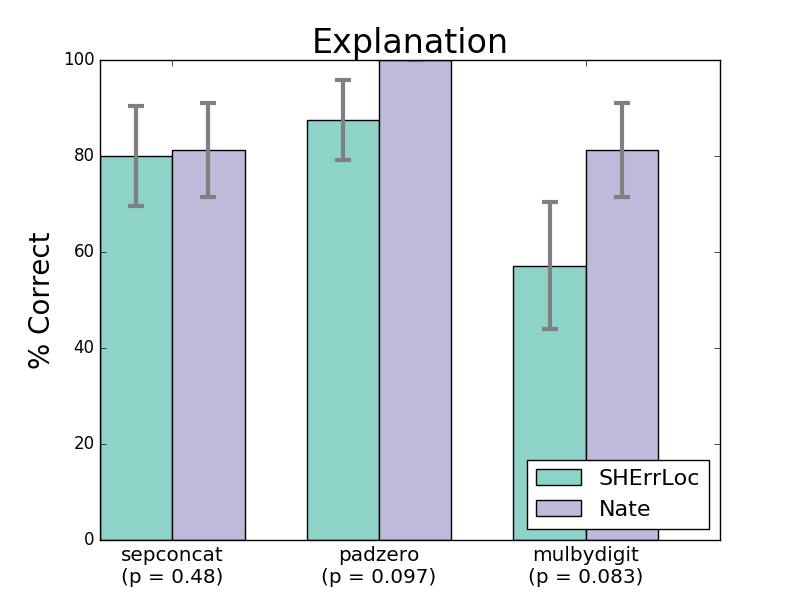
\includegraphics[width=0.7\linewidth]{nate/user-study-reason.png}
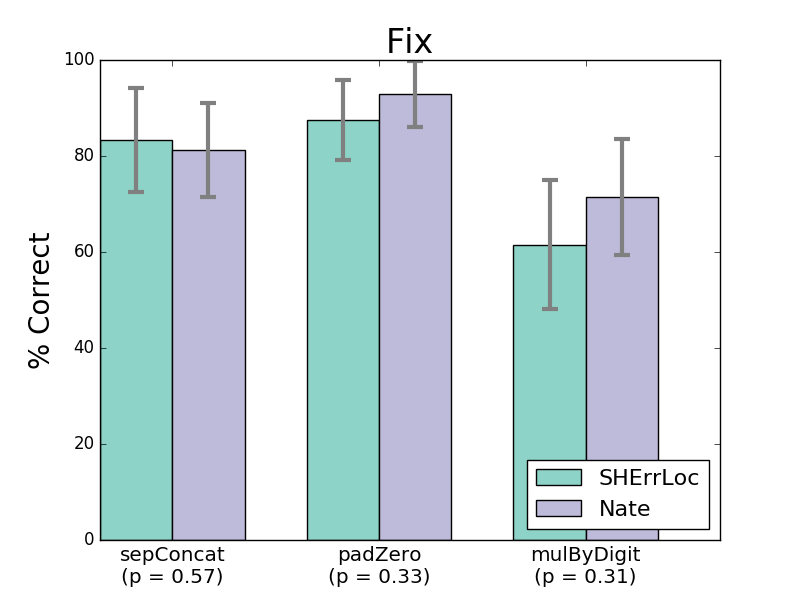
\includegraphics[width=0.7\linewidth]{nate/user-study-fix.png}
% \end{minipage}
% }
% \vspace{3ex}
\caption{A classification of students' explanations and fixes for type
  errors, given either \sherrloc or \toolname's blame assignment.
  %
  The students given \toolname's location generally scored
  better than those given \sherrloc's.
  %
  We report the result of a one-sided Mann-Whitney $U$ test for
  statistical significance in parentheses.}
\label{fig:results-user-study}
\end{figure}

\paragraph{Results}
%
The measured kappa values were $\kappa = 0.68$ for the explanations and
$\kappa = 0.77$ for the fixes; while there is no formal notion for what
consititutes strong agreement~\cite{Krippendorff2012-wd}, kappa values
above $0.60$ are often called ``substantial''
agreement~\cite{Landis1977-ey}.
%
Figure~\ref{fig:results-user-study} summarizes a single annotator's
results, which show that students given \toolname's blame assignment
were generally more likely to correctly explain and fix the type error
than those given \sherrloc's.
%
While there was no discernible difference between \toolname and
\sherrloc for |sepConcat|, \toolname responses for |padZero| and
|mulByDigit| were marked correct 5--30\% more often than the \sherrloc
responses.
%
The results appear to show a trend in favor of \toolname;
%
however, they are not statistically significant so
we cannot discount the possibility of confounding factors.
%


%%% Local Variables:
%%% mode: latex
%%% TeX-master: "main"
%%% End:

%% NUKE \mysection{Limitations}
\label{sec:nate:discussion}

We have shown that we can outperform the state of the art in type error
localization by learning a model of the errors that programmers make,
using a set of features that closely resemble the information the type
checker sees.
%
% However, there is certainly room for improvement.
%
In this section we highlight some limitations of our approach and
potential avenues for future work.

% \mysubsection{Limitations}
% \label{sec:nate:limitations}

\paragraph{User-Defined Types}
Probably the single biggest limitation of our technique is that we have
(a finite set of) features for specific data and type constructors.
%
Anything our models learn about errors made with the |::| constructor or
the |list| type cannot easily be translated to new, user-defined
datatypes the model has never encountered.
%
We can mitigate this, to some extent, by adding generic
syntactic features for data constructors and match expressions, but it
remains to be seen how much these help. % \ES{TODO: UW data!}.
%
Furthermore, there is no obvious analog for transferring knowledge to
new type constructors, which we have seen are both more compact and
helpful.

As an alternative to encoding information about \emph{specific}
constructors, we might use a more abstract representation.
%
For example, instead of modeling |x :: 2| as a |::| constructor with a
right child of type |int|, we might model it as some (unknown) constructor
whose right child has an incompatible type.
%
We might symmetrically model the |2| as an integer literal whose type is
incompatible with its parent.
%
Anything we learn about |::| and |2| can now be transferred directly to
yet unseen types, but we run the risk generalizing \emph{too much} ---
\ie perhaps programmers make different mistakes with |list|s than they
do with other types, and are thus likely to choose different fixes.
%
Balancing the trade-off between specificity and generalizability appears
to be a challenging task.

% \begin{itemize}
% \item Hard to support in general, as each data and type constructor gets
%   its own set of syntactic features.
% \item Attempt to mitigate by adding generic ``is-datacon'' and
%   ``is-match'' feature, unclear how much it will help
% \end{itemize}

\paragraph{Additional Features}
There are a number of other features that could improve the model's
ability to localize errors, that would be easier to add than
user-defined types.
%
For example, each occurrence of a variable knows only its type and its
immediate neighbors, but it may be helpful to know
about \emph{other} occurrences of the same variable.
%
If a variable is generally used as a |float| but has a
single use as an |int|, it seems likely that the
latter occurrence (or context) is to blame.
%
Similarly, arguments to a function application are not aware of the
constraints imposed on them by the function (and vice versa),
they only know that they are occurring in the context of an application.
%and the type of the application itself.
%
Finally, \emph{n-grams} on the token stream have proven effective for
probabilistic modeling of programming languages
\citep{Hindle2012-hf,Gabel2010-el}, we may find that they aid in
our task as well.
%
For example, if the observed tokens in an expression diverge from the
n-gram model's predictions, that indicates that there is something
unusual about the program at that point, and it may signal an error.

% \begin{itemize}
% \item def-use chains
% \item connect function and arguments in application (right now each only know about the application itself)
% \item ??
% \end{itemize}

\paragraph{Independent vs Joint Predictions}
We treat each sub-expression as if it exists in a vacuum, but in reality
the program has a rich \emph{graphical} structure, particularly if one adds
edges connecting different occurrences of the same variable.
%
\citet{Raychev2015-jg} have used these richer models to great effect to
make \emph{interdependent} predictions about programs, \eg
de-obfuscating variable names or even inferring types.
%
One could even view our task of locating the source of an error as simply
another property to be predicted over a graphical model of the program.
%
One of the key advantages of a graphical model is that the predictions
made for one node can influence the predictions made for another node,
this is known as \emph{structured learning}.
%
For example, if, given the expression |1 + true|, we predict |true| to
be erroneous, we may be much less likely to predict |+| as erroneous.
%
We compensate somewhat for our lack of structure by adding contextual
features and by ranking our predictions by ``confidence'', but it would
be interesting to see how structured learning over graphical models
would perform.


%%% Local Variables:
%%% mode: latex
%%% TeX-master: "main"
%%% End:

\section{Related Work}
\label{sec:nanomaly:related-work}
% In this section we connect our work to related efforts on type errors,
% testing, and program exploration.

% \paragraph{Type Errors}
% \label{sec:nanomaly:type-error}

\paragraph{Localizing and Repairing Type Errors}
\label{sec:nanomaly:diagnosis-repair}
% It is well known that
% unification-based type inference procedures can
% produce poor error messages, and in particular, can misidentify the
% \emph{source} of the type error.
%
Many groups have explored techniques to pinpoint the true source
of errors reported by static type checkers.
% unification-based type inference procedures.
%
% \subparagraph{Localization}
The traditional Damas-Milner type inference algorithm~\cite{Damas1982-uw}
reports the first program location where a type mismatch is discovered
(subject to the traversal strategy~\cite{Lee1998-ys}).
%
As a result the error can be reported far away from its
source~\cite{McAdam1998-ub} without enough information to guide the
user.
%
Type-error slicing~\cite{Haack2003-vc,Schilling2011-yf,Rahli2015-tt,Sagonas2013-bf,Gast2004-zd,Neubauer2003-xv}
%treats type inference as a constraint-satisfaction problem and
recognizes this flaw and instead produces a slice of the program
containing \emph{all} program locations that are connected to the type
error.
%
%% \cite{Neubauer2003-xv} present a decidable type system based on
%% discriminative sum types, in which all terms are typeable and type
%% derivations contain all type errors in a program. They then use the
%% typing derivation to slice out the parts of the expression related to
%% each error.
%
Though the program slice must contain the source of the error, it can
suffer from the opposite problem of providing \emph{too much}
information, motivating recent work in ranking the candidate locations.
%
Zhang~\etal~\citealt{Zhang2014-lv,Zhang2015-yu} present an algorithm for
identifying the most likely culprit using Bayesian reasoning.
%
Pavlinovic~\etal~\citealt{Pavlinovic2014-mr,Pavlinovic2015-kh}
translate the %error
localization problem to a MaxSMT optimization problem, using
compiler-provided weights to rank the possible sources.
%
Loncaric~\etal~\citealt{Loncaric2016-uk} improve the scalability of
Pavlinovic~\etal by reusing the existing type checker as
a theory solver in the Nelson-Oppen~\citealt{Nelson1979-td}
style, thus requiring only a MaxSAT solver.

% \subparagraph{Repairing}
In addition to localizing the error, Lerner~\etal~\citealt{Lerner2007-dt} attempt to
suggest a fix by replacing expressions (or removing them entirely) with
alternatives based on the surrounding program context.
%
Chen~\&~Erwig~\citealt{Chen2014-gd} use a variational type system to allow for the
possibility of changing an expression's type, and search for an
expression whose type can be changed such that type inference would
succeed.
%
% It then attempts to deduce the error source by searching for an
% expression whose type can be changed such that type inference would
% succeed.
%
In contrast to Lerner~\etal, who search for changes at the value-level,
Chen~\&~Erwig search at the type-level and are thus complete due the finite
universe of types used in the program.
%
% \item \cite{chen_error-tolerant_2012}
% \item \cite{okeefe_type_1992}
% \item \cite{gomard_partial_1990}
% \item \cite{thatte_type_1988}
%

In contrast to these approaches, we do not attempt to localize or fix
the type error. Instead we try to explain it to the user using a
dynamic witness that demonstrates how the program is not just
ill-typed but truly wrong. In addition, allowing users to run their
program (even knowing that it is wrong)
enables experimentation and the
use of debuggers to step through the program and investigate its
evolution.

\paragraph{Improving Error Messages}
%
The content and quality of the error messages themselves has also been
studied extensively.
%
Marceau~\etal~\citealt{Marceau2011-ok,Marceau2011-cy} study the effectiveness of error
messages in novice environments and present suggestions for improving
their quality and consistency.
%
Hage~\&~Heeren~\citealt{Hage2006-hc} identify a variety of general heuristics to improve
the quality of type error messages, based on their teaching experience.
%
Heeren~\etal~\citealt{Heeren2003-db},
Christiansen~\citealt{Christiansen2014-qc}, and
Serrano~\&~Hage~\citealt{Serrano2016-oo}
provide methods for library authors to specialize
type errors with domain-specific knowledge.
%
The difference with our work is more pronounced here as we do not
attempt to improve the quality of the error message, instead we search
for a witness to the error and explain it with the resulting execution
trace.
%



\paragraph{Running Ill-Typed Programs}
\label{sec:nanomaly:running-ill-typed}
Vytiniotis~\etal~\citealt{Vytiniotis2012-gh} extend the \haskell
compiler GHC to support compiling ill-typed programs, but their intent
is rather different from ours. Their goal was to allow programmers to
incrementally test refactorings, which often cause type errors in
distant functions. They replace any expression that fails to type
check with a \emph{runtime} error, but do not check types
at runtime.
%
Bayne~\etal~\citealt{Bayne2011-cn} also provide a semantics for running
ill-typed (\java) programs, but in constrast transform the program to
perform nearly all type checking at run-time. The key difference between
Bayne~\etal\ and our work is that we use the dynamic semantics to
automatically search for a witness to the type error, while their focus
is on incremental, programmer-driven testing.

\paragraph{Testing}\label{sec:nanomaly:testing}
%
\nanomaly is at its heart a test generator, and as such,
builds on a rich line of work.
%
Our use of holes to represent unknown values is inspired by the work of
Runciman, Naylor, and Lindblad~\cite{Runciman2008-ka,Naylor2007-mi,Lindblad2007-oy},
%
who use lazy evaluation to drastically reduce the search space for
exhaustive test generation, by grouping together equivalent inputs by
the set of values they force. An exhaustive search is complete (up to
the depth bound), if a witness exists it will be found, but due to the
exponential blowup in the search space the depth bound can be quite
limited without advanced grouping and filtering techniques.
%
Our search is not exhaustive; instead we use random generation to fill
in holes on demand.
%
Random test generation~\cite{Claessen2000-lj,Csallner2004-bf,Pacheco2007-at}
%
is by its nature incomplete, but is able to check larger inputs than
exhaustive testing as a result.

Instead of enumerating values, which may trigger the same path through
the program, one might enumerate paths.
%
Dynamic-symbolic execution~\cite{Godefroid2005-am,Cadar2008-kg,Tillmann2008-qc}
%
combines symbolic execution (to track which path a given input triggers)
with concrete execution (to ensure failures are not spurious). The
system collects a path condition during execution, which tracks
symbolically what conditions must be met to trigger the current
path. Upon successfully completing a test run, it negates the path
condition and queries a solver for another set of inputs that satisfy
the negated path condition, \ie inputs that will not trigger the same
path. Thus, it can prune the search space much faster than techniques
based on enumerating values, but is limited by the expressiveness of the
underlying solver.

Our operational semantics is amenable to dynamic-symbolic execution, one
would just need to collect the path condition and replace our
implementation of \gensym by a call to the solver. We chose to use lazy,
random generation instead because it is efficient, does not incur
the overhead of an external solver, and produces high coverage for our
domain of novice programs.

A function's type is a theorem about the its behavior.
Thus, \toolname's witnesses can be viewed as \emph{counter-examples},
thereby connecting it to work on using test cases to find
counter-examples prior to starting a proof~\cite{Chamarthi2011-fo,Seidel2015-pe}.

% \begin{itemize}
% \item \cite{Claessen2000-lj}
% \item
% \item \cite{Godefroid2005-am}
% \item \cite{Cadar2008-kg}
% \item \cite{Tillmann2008-qc}
% \end{itemize}

\paragraph{Program Exploration}

Flanagan~\etal~\citealt{Flanagan1996-bu} describe a static debugger for Scheme, which helps
the programmer interactively visualize problematic source-sink flows
corresponding to soft-typing errors. The debugger allows the user to explore
an abstract reduction graph computed from a static value set analysis of
the program. In contrast, \toolname generates witnesses and allows the user
to explore the resulting dynamic execution.
%
Perera~\etal~\citealt{Perera2012-dy} present a tracing semantics
for functional programs that tags values with their provenance, enabling
a form of backwards program slicing from a final value to the sequence
of reductions that produced it. Notably, they allow the user to supply a
\emph{partial value} --- containing holes --- and present a partial slice,
containing only those steps that affected the the partial value.
% This
% system is designed to answer questions of the form ``Where did this
% value come from?'' and thus is focused on backward exploration.
Perera~\etal\ focus on backward exploration; in contrast, our
visualization supports forward \emph{and} backward exploration, though
our backward steps are more limited.
%
Specifically, we do not support selecting a value and inserting the
intermediate terms that preceded it while ignoring unrelated computation
steps. %; this would be interesting future work.

% \ES{todo: more on program exploration}

%%% Local Variables:
%%% mode: latex
%%% TeX-master: "../main"
%%% End:


\subsection*{Acknowledgements}
This work was supported by NSF grants CCF-1422471,
CNS-0964702, CNS-1223850, CCF-1218344, CCF-1018672, and
a generous gift from Microsoft Research.
We thank 
Lee Pike
and the reviewers for their 
excellent feedback on
a draft of this paper.

{
\bibliographystyle{splncs03}
\bibliography{sw}
}

\includeTechRep{
  \appendix
  \section{Instantiating \toolname Generically}\label{sec:genericapp}

\GhcGenerics defines separate types for products, data constructors, sums, and
datatypes; and uses the @TypeFamilies@ extension~\cite{Chakravarty_ATS_2005} to define an 
associated generic representation @Rep a@ for any algebraic datatype. For 
example, the standard Haskell list would be represented by the generic type
%
\begin{code}
  Rep [a] = C1 U1 :+: C1 (Rec0 a :*: Rec0 [a])
\end{code}
%
where @C1@ denotes a data constructor, @U1@ an empty product (\eg for a nullary
constructor), @:+:@ a sum, and @:*:@ a product. Additionally, @Rec0@ indicates a
reference to a user-defined type, \ie values are translated to and from the
universal representation \emph{as-needed}. We omit some of the metadata to
highlight the structural similarity between the generic representation and the
original data definition.

\ES{TODO: explain that insight of ghc-generics is that you can treat all sums
  equally and all products equally, so general approach is to define two
  type-classes: one that handles sums and another that handles products.}

\ES{TODO: explain that generic rep is tree-structured, NOT list.}

% 3 type-specific pieces of overall approach:
%   1. obtaining list of @Con@s to unfold at a given depth
%   2. decoding a specific @Con@
%   3. encoding a @Con@ 

Recall that our implementation from \S~\ref{sec:list} contained three
pieces of type-specific logic, namely
%
(1) obtaining a list of @Ctor@s to unfold at a given depth (@ctors@),
%
(2) decoding a specific @Ctor@ (@decodeCtor@), and
%
(3) encoding a Haskell value as a logical expression (@encode@).
%
We now demonstrate how to generically implement these three steps for any
algebraic datatype, but first we will need two extensions to our refinement type
API, which we describe in Figure~\ref{fig:rtype-ext}.

\begin{figure}
\begin{mdframed}
\begin{CenteredBox}
\begin{code} 
ctorArity :: Ctor -> Int
mkCtor    :: Proxy (C1 c f) -> Ctor
\end{code}
\end{CenteredBox}
\end{mdframed}
\caption{Extensions to the refinement type API from Figure~\ref{fig:rtype}}\label{fig:rtype-ext}
\end{figure}

\begin{itemize}
\item{@ctorArity@} returns the number of fields that a @Ctor@ has.
\item{@mkCtor@} constructs a @Ctor@ from a \emph{proxy} for the constructor.
\end{itemize}

\subsection{Listing Constructors}\label{sec:generic-constructors}
Let us begin by writing a function @gCtors@ that will work just like @ctors@,
but for any datatype, \ie it will return a list of @Ctor@s that should be
unfolded at the given depth @d@. As is standard for \GhcGenerics we will define
a type-class for @gCtors@ and provide instances for sums, products, etc.
\GhcGenerics uses a number of different types for which we must provide class
instances, but only a few of the instances are interesting, which we show in
Figure~\ref{fig:generic-query}.
%
\begin{figure}[ht]
\begin{mdframed}
\begin{CenteredBox}
\begin{code}
  class GCtors f where
    gCtors :: Proxy f -> Int -> [Ctor]

  instance (GCtors f, GCtors g) => GCtors (f :+: g) where
    gCtors _ d = gCtors (Proxy :: Proxy f) d 
              ++ gCtors (Proxy :: Proxy g) d

  instance GCtors f => GCtors (C1 c f) where
    gCtors p 0
      | conArity c == 0 = [c]
      | otherwise       = []
      where
        c = mkCtor p
    gCtors p d
      = [mkCtor p]
\end{code}
\end{CenteredBox}
\end{mdframed}
\caption{Generic query generation}\label{fig:generic-query}
\end{figure}
%
For example, to obtain the list of @Ctor@s for a sum we simply concatenate the
lists obtained from the left- and right-hand sides of the sum.  When we reach a
specific constructor, we compare the constructor's arity with the depth; when we
reach depth 0 we only want to unfold \emph{nullary} constructors~\footnote{In
  practice one might want to do something smarter, like checking the minimum
  depth required to unfold the constructor.}.
\ES{The (C1 c f) might be confusing because the "c" was omitted in the "Rep [a]"
  example above...}
Now we can replace the call to @ctors@ in @queryList@ with
%
\begin{code}
  -- reproxyRep :: Proxy a -> Proxy (Rep a)
  let cs = gCtors (reproxyRep $ proxy t) d
\end{code}
%
\ES{i'm pretty sure (reproxyRep \$ proxy t) won't typecheck due to the existential..}
making our @query@ implementation fully datatype-generic.

% instance GCons f => GCons (D1 d f) where
%   gCons _ d = gCons (Proxy :: Proxy f) d

% class GHasDepth f where
%   gHasDepth :: Proxy f -> Int -> Bool

% instance (GHasDepth f, GHasDepth g) => GHasDepth (f :*: g) where
%   gHasDepth _ d = gHasDepth (Proxy :: Proxy f) d 
%                && gHasDepth (Proxy :: Proxy g) d

% instance GHasDepth U1 where
%   gHasDepth _ _ = True
  
% instance GHasDepth (Rec0 a) where
%   gHasDepth _ 0 = False
%   gHasDepth _ _ = True

\subsection{Decode}\label{sec:generic-decode}
Next we will tackle the process of \emph{decoding} a specific constructor from
the model. As above, we will define a type-class and show only the interesting
instances in Figure~\ref{fig:generic-decode}.
%
\begin{figure}[ht]
\begin{mdframed}
\begin{CenteredBox}
\begin{code}
  class GDecode f where
    gDecode :: Ctor -> [Var] -> Gen f

  instance (GDecode f, GDecode g) => GDecode (f :+: g) where
    gDecode c vs =  L1 <$> gDecode c vs
                <|> R1 <$> gDecode c vs

  instance GDecodeFields f => GDecode (C1 c f) where
    gDecode c vs 
      | c == mkCtor (Proxy :: Proxy (C1 c f))
      = C1 . snd <$> gDecodeFields vs
      | otherwise
      = empty

  class GDecodeFields f where
    gDecodeFields :: [Var] -> Gen ([Var], f)

  instance Targetable a => GDecodeFields (Rec0 a) where
    gDecodeFields (v:vs) = do
      x <- decode v
      return (vs, Rec0 x)
\end{code}
\end{CenteredBox}
\end{mdframed}
\caption{Generic decoding of Haskell values}\label{fig:generic-decode}
\end{figure}

Given an arbitrary sum, we do not know whether the constructor we are looking
for is in the left or right sub-sum, so we must try both.
%
Once we reach an individual constructor, we can check whether it is the correct
constructor using the forementioned @mkCtor@ function. If the check is
successful, we can go ahead and decode the constructor's fields using
@gDecodeFields@ and wrap them up, otherwise we signal that the next element of
the sum should be tried.

@gDecodeFields@ comes from an auxiliary type-class that we use to decode the
fields of a product. As \GhcGenerics represents sums and products as
\emph{trees} instead of lists, we have @gDecodeFields@ return the list of
@Var@s that still need to be decoded in addition to the decoded value.
%
Again, most of the instances are uninteresting and simply involve traversing the
product while decoding each field. The interesting instance arises when we want
to encode an individual field. Recall that products are represented with
recursive references to the user-defined type, \eg @Rec0 [a]@. So when we reach
an individual field, we will have to decode a value of the \emph{user-defined}
type.

We can now replace the @decodeCtor c fs'@ in our original implementation of @decode@
with
%
\begin{code}
  -- to :: Generic a => Rep a -> a
  to <$> gDecode c xs
\end{code}
%
% instance GDecode f => GDecode (D1 d f) where
%   gDecode c vs = D1 <$> gDecode c vs
%
% instance (GDecodeFields f, GDecodeFields g) => GDecodeFields (f :*: g) where
%   gDecodeFields vs = do
%     (vs', ls)  <- gDecodeFields vs
%     (vs'', rs) <- gDecodeFields vs'
%     return (vs'', ls :*: rs)
%     
% instance GDecodeFields U1 where
%   gDecodeFields vs = return (vs, U1)
%
\subsection{Check}\label{sec:generic-check}
Finally, let us examine how to generically \emph{check} that Haskell value 
inhabits a refinement type with the type-class in Figure~\ref{fig:generic-check}.
%
\begin{figure}[ht]
\begin{mdframed}
\begin{CenteredBox}
\begin{code}
  class GCheck f where
    gCheck :: f -> RefType -> Gen (Bool,Var)
    
  class GCheckFields f where
    gCheckFields :: f -> [(Var, RefType)]
                 -> SMT (Bool, [Var], [(Var, RefType)])
                 
  instance GCheckFields f => GCheck (C1 c f) where
    gCheck (C1 f) t = do
      let c       = mkCtor (Proxy :: Proxy (C1 c f))
      let fts     = unfold c t
      (b, vs, _) <- gCheckFields f fts
      v          <- apply c vs
      let t'      = t `subst` [(binder t, v)]
      b'         <- eval t'
      return (b', v)
      
  instance Targetable a => GCheckFields (Rec0 a) where
    gCheckFields (Rec0 a) ((f, t) : fts) = do
      (b, v)  <- check a t
      let fts' = fts `subst` [(f, v)]
      return (b, [v], fts')
\end{code}
\end{CenteredBox}
\end{mdframed}
\caption{Generic checking of Haskell values against refinement types.}\label{fig:generic-check}
\end{figure}

Checking a sum just involves stripping away levels of indirection until we reach
the actual constructor, at which point we need to unfold the constructor and
check its fields. We then @apply@ the constructor to the resulting symbolic
values, @subst@itute the resulting @Refinement@ for @t@'s @binder@ and
@eval@uate the result.

@gCheckFields@ checks the fields of a product, and is itself a type-class method.
%
As with @gDecodeFields@ the only interesting instance of @GCheckFields@ deals
with checking an individual field, where we have a value of the user-defined
type and must use the original @check@ method.

Now we can provide a default implementation for @check@
%
\begin{code}
  -- from :: Generic a => a -> Rep a
  check v t = gCheck (from v) t
\end{code}
%
thus replacing the last bit of type-specific logic in our @Targetable@
implementation.

% instance GEncode f => GEncode (D1 d f) where
%   gEncode (D1 f) t = gEncode f t

% instance (GEncode f, GEncode g) => GEncode (f :+: g) where
%   gEncode (L1 f) = gEncode f
%   gEncode (R1 g) = gEncode g

% instance (GEncodeFields f, GEncodeFields g) => GEncodeFields (f :*: g) where
%   gEncodeFields (f :*: g) ts = do
%     (fs,ts')  <- gEncodeFields f ts
%     (gs,ts'') <- gEncodeFields g ts'
%     return (fs ++ gs, ts'')

% instance GEncodeFields U1 where
%   gEncodeFields U1 = []


%%% Local Variables:
%%% mode: latex
%%% TeX-master: "main"
%%% End:

}

\end{document}

%%% Local Variables: 
%%% mode: latex
%%% TeX-master: "main"
%%% End: 
